% !TEX root = ./rosbook_jp.tex
%-------------------------------------------------------------------------------
\chapterimage{chapter_head_10.pdf}

%-------------------------------------------------------------------------------
\chapter{SLAMとナビゲーション}\index{SLAMとナビゲーション}

SLAM (Simultaneous Localization And Mapping)とは、ロボットが未知の環境を移動しながら、ロボットに搭載されたセンサだけで自己位置を推定し、同時に走行経路や障害物などの地図を作成する技術である。LRFやデプスセンサの開発により、SLAMは近年、盛んに研究され、急速に発展している。一方、ナビゲーション (navigation)とは、地図が与えられた時に、出発地から目的地へロボットを安全に移動させる技術である。SLAM、ナビゲーションともに、移動ロボットでは最も基本的で重要な技術であり、本章ではROSを用いたSLAMやナビゲーションの実現方法を説明する。

%-------------------------------------------------------------------------------
\section{ナビゲーションに必要な機能}\index{ナビゲーションに必要な機能}

本節では、移動ロボットのナビゲーションに必要な4つの機能について説明する。ナビゲーションは、広義には出発地から目的地まで人やものを案内する機能である。我々にとって最も身近なナビゲーションは、カーナビゲーションシステム (カーナビ)であろう。カーナビは、端末の地図上で目的地を設定すると、現在位置から目的地までの正確な距離、所要時間、経由する場所や利用する道路などを詳細に表示してくれる。
移動ロボットにおけるナビゲーションは、図10-1に示すように出発地から目的地まで、“障害物を避けながら”移動する機能である。ナビゲーションは古くから研究されており、これまでに様々な手法が提案されてきた  。

\begin{figure}[htp]
  \centering
  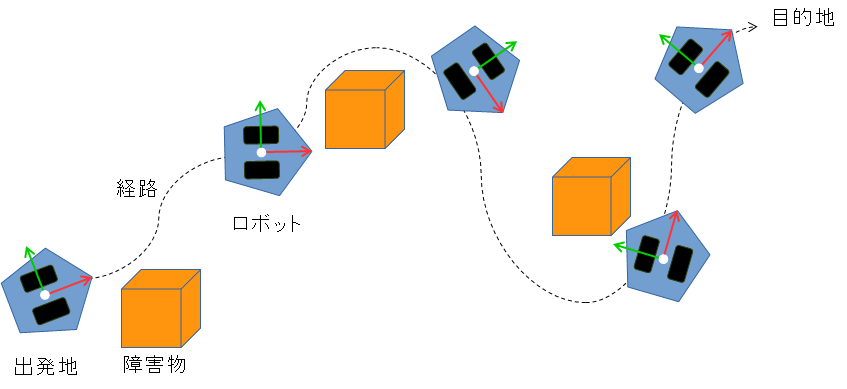
\includegraphics[width=15cm]{pictures/chapter10/pic_10_01.png}
  \caption{ナビゲーション}
\end{figure}

移動ロボットのナビゲーションには、次の要素  が必須である。

\setcounter{num}{0}

\stepcounter{num}\circled{\thenum} 移動のための地図   (環境地図)
\stepcounter{num}\circled{\thenum} 移動中のロボットの位置計測/推定機能
\stepcounter{num}\circled{\thenum} 壁、家具、人などを避けて移動する障害物回避
\stepcounter{num}\circled{\thenum} 現在地から目標地までの効率的な経路探索

これら4つの要素について、次項以降で詳しく説明する。

%-------------------------------------------------------------------------------
\subsection{移動のための地図 (環境地図)}

カーナビの役割は車の運転者に目的地までの道案内をすることであり、これはシステムに搭載された地図に基づいて行われる。 移動ロボットのナビゲーションにおいても同様に、現在地と目的地を含む正確な地図,すなわち環境地図が必要である。  環境地図はあらかじめ人手により用意するか、ロボットが自ら作成する必要がある。
環境地図を人手により用意する場合は、屋内であれば建築図面や家具の配置図、屋外であれば道路地図などを用いて、ロボットが走行可能な経路をあらかじめ決定しておく。しかし、人手による環境地図の作成には手間がかかり、また例えば家具の配置が変われば、再度作成しなおす必要がある。
一方、移動ロボットが自ら環境地図を作成する方法として、近年、SLAMが盛んに研究されてきた。SLAMとは、前述のように、ロボットが未知の空間を移動する際、LRFやカメラで周囲の環境情報を取得し、自らの現在位置を推定すると同時に、環境地図も作成する方法である。SLAMについて詳しくは10.4節で説明する。

%-------------------------------------------------------------------------------
\subsection{移動中のロボットの位置計測/推定機能}

ナビゲーションにおいて、移動ロボットが自己位置を計測/推定する機能は必須である。移動ロボットにおける最も基本的な自己位置計測手法は、車輪の回転量を用いるオドメトリ (odometry)法  である。しかしオドメトリ法は、車輪の滑りなどによって誤差が蓄積されやすい。そこで、IMUセンサなどで慣性情報 (速度や加速度)を取得し、それらの情報を統合することで誤差の蓄積を低減する方法がしばしば用いられる。オドメトリ法やIMUセンサを用いた方法など、微少な移動量を加え合わせて現在位置を推定する手法をデッドレコニング法 (dead reckoning)と呼ぶ。

\begin{figure}[htp]
  \centering
  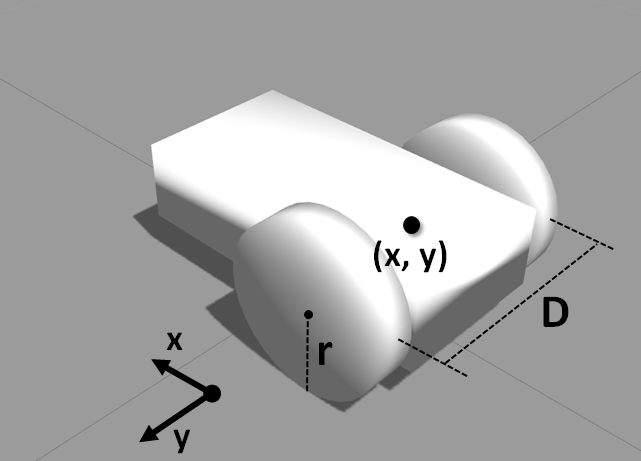
\includegraphics[width=8cm]{pictures/chapter10/pic_10_02.png}
  \caption{オドメトリ法に必要な情報 (中心位置座標 (x、y)、車輪間の距離D、車輪半径r)}
\end{figure}

図10-2のように2つの車輪を持つ移動ロボットを例に、オドメトリ法について説明する。図10-3のように、時間$T_e$の間に移動ロボットが微少距離だけ移動したとする。車輪間の距離をD、車輪の半径をrとすると、左右のモータ回転量 (現在のエンコーダ値$E_lc$,$E_rc$と$T_e$時刻前のエンコーダ値$E_lp$, $E_rp$)を用いて、左右の車輪の回転速度が式10-1、10-2として求まる。

\begin{equation}
v_lk = ((E_lc-E_lp)/T_e) π/180     (radian/sec)
\end{equation}

\begin{equation}
v_rk = ((E_rc-E_rp)/T_e)π/180     (radian/sec)
\end{equation}

次に、式10-3、10-4により左右の車輪の移動速度を求め、式10-5、10-6より   移動ロボットの並進速度 (v)と回転角速度 (ω)を求める。

\begin{equation}
V_l = v_lk r     (meter/sec)
\end{equation}

\begin{equation}
V_r = v_rk r     (meter/sec)
\end{equation}

\begin{equation}
v_k = (V_rk+V_lk)/2     (meter/sec)
\end{equation}

\begin{equation}
\omega_k=(V_rk-V_lk)/D     (radian/sec)
\end{equation}

最後にそれらを現在の値に足し合わせて、式10-7~10-10のように移動後の位置と姿勢を求める。

\begin{equation}
\Delta s=v_k T_e
\Delta\theta=\omega_k T_e
\end{equation}

\begin{equation}
x_(k+1)=x_k+\Delta s \cos(\theta_k+\Delta\theta/2)
\end{equation}

\begin{equation}
y_(k+1)=y_k+\Delta \sin(\theta_k+\Delta\theta/2)
\end{equation}

\begin{equation}
\theta_(k+1)=\theta_k+\Delta\theta
\end{equation}

%-------------------------------------------------------------------------------
\subsection{壁、家具、人などを避けて移動する障害物回避}

移動ロボットは人間が操縦するカーナビと違い、ロボットが自ら移動中に障害物を検出して、衝突を回避しなければならない。障害物には壁、家具などの静止したものと、人や車など移動するものがあるが、それらの検出には、遠距離から非接触で存在を検出できる距離センサやビジョンセンサが利用される。距離センサには、LRF、超音波センサ、赤外線距離センサなどが良く用いられる。一方、ビジョンセンサには、単眼カメラ、ステレオカメラ、全方位カメラなどがあり、最近ではKinect、Xtionなどのデプスカメラも広く利用されている。  検出された障害物情報を基に、次項の最適経路の計算手法により、適切な回避動作が計画される。

\begin{figure}[htp]
  \centering
  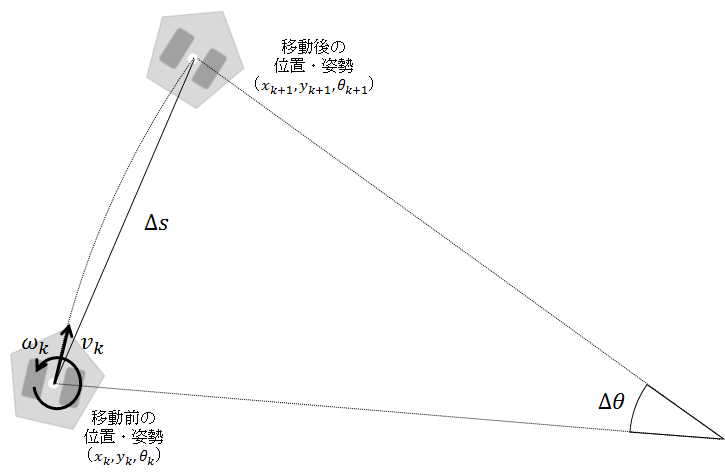
\includegraphics[width=12cm]{pictures/chapter10/pic_10_03.png}
  \caption{オドメトリ法}
\end{figure}

%-------------------------------------------------------------------------------
\subsection{最適経路の計算}

目的地までの最適な経路を探索する機能は経路探索/経路計画と呼ばれ、ダイクストラ法、A*アルゴリズム、ポテンシャル法、RRT (Rapidly exploring Random Tree)など、様々な方法がある。

%-------------------------------------------------------------------------------
\section{ROSを用いたSLAMの実行手順}\index{ROSを用いたSLAMの実行手順}

10.1.1項で、ロボットが自ら環境地図をつくる手法としてSLAMがあると述べた。本節では、ROSとKobukiを利用したSLAMの実行手順について説明する。SLAMのアルゴリズムや要素技術は、10.3節以降で詳しく説明する。

%-------------------------------------------------------------------------------
\subsection{ロボットハードウェアの制約}

本節では、SLAMのアルゴリズムとして公開されているGmapping注1を利用する。 Gmappingを利用するには、ハードウェアに以下のような制約がある。

\setcounter{num}{0}

\stepcounter{num}\circled{\thenum} 移動コマンド

使用する移動ロボットは、以下のいずれかでなければならない。

\begin{itemize}
\item 2個の車輪と2個の駆動モータを有し、左右車輪が別々に駆動可能な差分駆動型移動ロボット
\item 全方向車輪であるオムニホイールを3つ以上備え、それぞれが別々の駆動モータで駆動される全方向移動ロボット
また、移動ロボットは、x、y軸の並進速度コマンドとz軸回りの回転角速度コマンドで動作しなければならない。
\end{itemize}

\stepcounter{num}\circled{\thenum} 自己位置情報

自己位置情報が得られなければならない。つまり、自身の移動量、回転量を、オドメトリ法やIMUセンサなどを用いて計測し、自己位置が推定できなければならない。

\stepcounter{num}\circled{\thenum} 搭載センサ

XY平面 (床面)上の障害物の位置、形状を正確に計測できるLRF、LiDARなどの2次元距離センサを備えなければならない。ただし、Kinect、Xtionのようなデプスカメラにより得られた3次元情報を、XY平面上の2次元距離情報に変換して用いることもできる。

\stepcounter{num}\circled{\thenum} ロボットの形態

正方形、長方形、円筒形 の車輪型移動ロボットでなければならない。一辺が極端に長いロボットや複雑な形状のロボット、2足ヒューマノイドロボット、多脚移動ロボット、飛行ロボット、水中ロボットなどは適用外である。
本節では、第9章で紹介した移動ロボットプラットフォームKobuki注2を使用する。ただし、図10-4に示すように、Kobuki本体にタートルボット2のモジュールプレートとフレームを2段に積んだ。下段にはノートパソコンを設置し、上段に北陽電機製 LRF注3  (UTM-30LX)を搭載した。ただし、本節ではKobukiプラットフォームとLRFを用いた場合について説明するが、これを応用すれば、特定のロボットプラットフォーム、特定のセンサに限らず、様々なロボットにSLAMを実装できる。

\begin{figure}[htp]
  \centering
  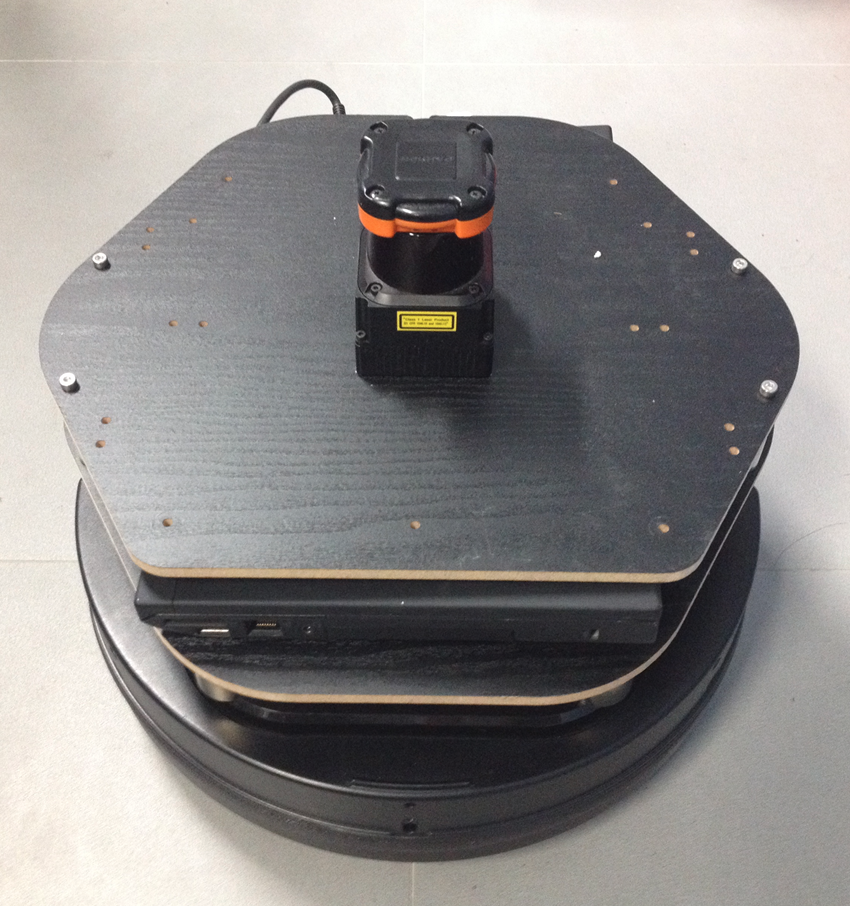
\includegraphics[width=8cm]{pictures/chapter10/pic_10_04.png}
  \caption{LRFを搭載したKobuki}
\end{figure}

%-------------------------------------------------------------------------------
\subsection{SLAMが利用できない環境}

SLAMは周囲の幾何的特徴を連続的に抽出し、追跡していく手法である。したがって、抽出すべき幾何的特徴のない空間では、SLAMを利用できない。特徴的な構造が非常に少ない環境として、例えば

\begin{itemize}
\item  障害物がなく形状が対称な  環境
\item 平行な2枚の壁に挟まれた長い廊下
\end{itemize}

が挙げられる。また、センサ情報が得られない環境、例えば

\begin{itemize}
\item 窓やガラス、黒い壁、水面、鏡などで囲まれた環境
\item 広大で壁や障害物が遠く、何も計測できない環境
\end{itemize}

などでは、SLAMを適用することができない。

%-------------------------------------------------------------------------------
\subsection{SLAMのためのROSパッケージ}

本章で使用するSLAM関連のROSパッケージは、kobukiメタパッケージと、slam\_gmappigメタパッケージに含まれるgmappingパッケージ、navigationメタパッケージに含まれるmap\_serverパッケージである。 本節では、SLAMの実行方法のみを記載し、各パッケージの仕様については、次節で詳しく述べる。以下で示すパッケージのインストール、ノードやlaunchファイルの実行はすべてKobuki本体と接続されたノートパソコンで行う必要がある。
まず、次のようにSLAM関連のROSパッケージをすべてインストールしておく。

\begin{lstlisting}[language=ROS]
$ sudo apt-get install ros-indigo-kobuki*
$ sudo apt-get install ros-indigo-gmapping
$ sudo apt-get install ros-indigo-navigation
\end{lstlisting}

ROSパッケージに加えて、センサパッケージも必要となる。使用するセンサに合わせた関連パッケージをインストールしよう。本節では、北陽電機製LRF (UTM-30LX)を用いるが、KinectやXtionのインストール法も参考までに記載している。
北陽電機製LRF (URG-04LXとUTM-30LXシリーズ)パッケージのインストールは、次のとおりである。

\begin{lstlisting}[language=ROS]
$ sudo apt-get install ros-indigo-urg-node
\end{lstlisting}

Kinectセンサパッケージのインストールは、次のとおりである。

\begin{lstlisting}[language=ROS]
$ sudo apt-get install ros-indigo-freenect*
\end{lstlisting}

また、Xtionセンサパッケージのインストールは、次のとおりである。

\begin{lstlisting}[language=ROS]
$ sudo apt-get install ros-indigo-openni2*
\end{lstlisting}

%-------------------------------------------------------------------------------
\subsection{SLAMの実行}

では、実際にKobukiとLRFを用いてSLAMを実行してみる。

\setcounter{num}{0}

\stepcounter{num}\circled{\thenum} ソースコードのダウンロードとビルド

まず、次のように関連パッケージをダウンロードする。次にcatkin\_makeコマンドを使用して、ダウンロードしたパッケージをビルドする。

\begin{lstlisting}[language=ROS]
$ cd ~/catkin_ws/src
$ git clone https://github.com/irvs/rosbook_kobuki.git
$ cd ~/catkin_ws && catkin_make
\end{lstlisting}

\stepcounter{num}\circled{\thenum} Kobukiノードの実行

roscoreを実行した後、新しいターミナルウィンドウを開き、Kobukiノードを実行する。kobuki\_ftdiパッケージやkobuki\_nodeパッケージは9.5節で説明したKobukiの起動に必要なパッケージである。

\begin{lstlisting}[language=ROS]
$ roscore
\end{lstlisting}

\begin{lstlisting}[language=ROS]
$ rosrun kobuki_ftdi create_udev_rules
$ roslaunch kobuki_node minimal.launch --screen
\end{lstlisting}

\stepcounter{num}\circled{\thenum} kobuki\_slamの実行

ノートパソコンをKobukiに接続し、ポートを設定する (9.6節参照)。次にkobuki\_s\\lam.launchファイルを実行する。このlaunchファイルは、LRFのドライバであるurg\_nodeノード、座標変換のためのkobuki\_tfノード、環境地図作成のためのslam\_gmappingノードの、計3つのノードを同時に起動する。

\begin{lstlisting}[language=ROS]
$ sudo chmod a+rw /dev/ttyACM0
$ roslaunch kobuki_slam kobuki_slam.launch
\end{lstlisting}

\stepcounter{num}\circled{\thenum} RVizの実行

SLAMの動作を確認するため、RVizを起動する。次のようにRVizにオプション (“-d `rospack find kobuki\_slam`/rviz/kobuki\_slam.rviz”)  を付けて起動すると、結果表示のためのプラグインが自動的に追加され、便利である。

\begin{lstlisting}[language=ROS]
$ rosrun rviz rviz -d `rospack find kobuki_slam`/rviz/kobuki_slam.rviz
\end{lstlisting}

\stepcounter{num}\circled{\thenum} トピックメッセージの保存

Kobukiとkobuki\_slamパッケージで配信する「/scan」と「/tf」トピックを、「scan\_\\data」というファイル名のbagファイルとして保存しておく。4.3.7項で説明したように、rosbagコマンドでトピックをファイルに保存しておくと、実行中の「/scan」と「/tf」トピックを実行後に再生でき、ロボットを実際に用いなくても環境地図の再作成が可能になる。

\begin{lstlisting}[language=ROS]
$ rosbag record -O scan_data /scan /tf
\end{lstlisting}

\stepcounter{num}\circled{\thenum} ロボットの操縦

次のコマンドで、ユーザーが直接ロボットを操作し、SLAMを実行する。操作する時、ロボットの速度を急に変えたり、急に回転させたりしてはいけない。計測対象の環境の隅々までロボットを移動させながら、LRFで計測する。

\begin{lstlisting}[language=ROS]
$ roslaunch kobuki_keyop safe_keyop.launch
\end{lstlisting}

\stepcounter{num}\circled{\thenum} 環境地図 作成

環境計測が終わったら、map\_saverノードを実行して環境地図を作成しよう。

\begin{lstlisting}[language=ROS]
$ rosrun map_server map_saver
\end{lstlisting}

map\_saverノードは、ロボットのオドメトリ情報、tf情報、LRFの距離情報から自動的に環境地図を作成する。作成された環境地図は、すでに起動しているRVizで確認できる。
実際に、図10-5に示す環境を用意し、環境地図を作成した。この環境には、ベッド、机、テーブル、棚、本棚、冷蔵庫、TV、ソファなどが含まれる。

\begin{figure}[htp]
  \centering
  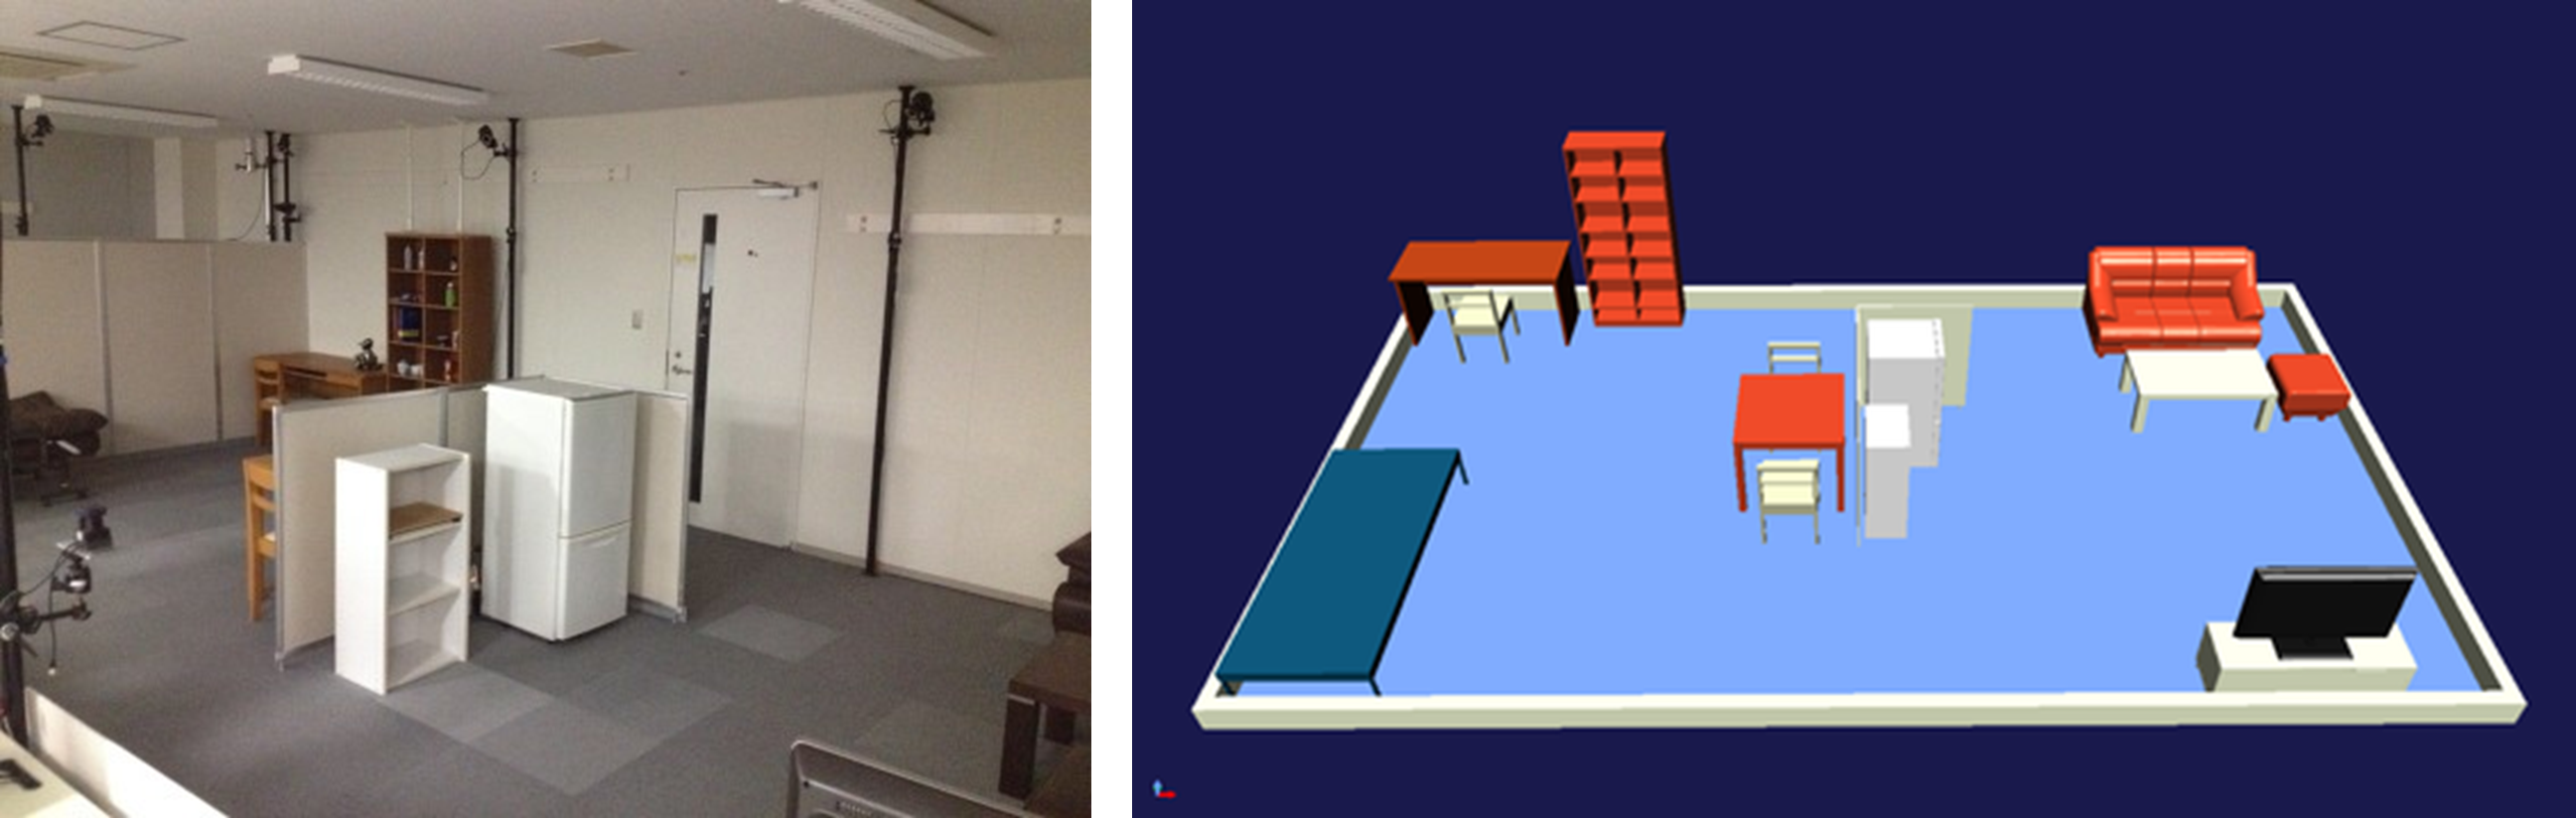
\includegraphics[width=12cm]{pictures/chapter10/pic_10_05.png}
  \caption{計測対象の環境 (左)と計測対象の3次元モデル (右)}
\end{figure}

図10-6に環境地図作成の途中経過を、図10-7に完成した環境地図を示す。図10-5で示した環境の環境地図が作成されたことを確認できる。なお、ファイル名を特に指定しなければ、map\_saverを動作させたディレクトリに、実際の環境地図であるmap.pgmファイルと、解像度などの情報を含むmap.yamlファイルが保存される。環境地図の保存形式については、10.3節で説明する。

\begin{figure}[htp]
  \centering
  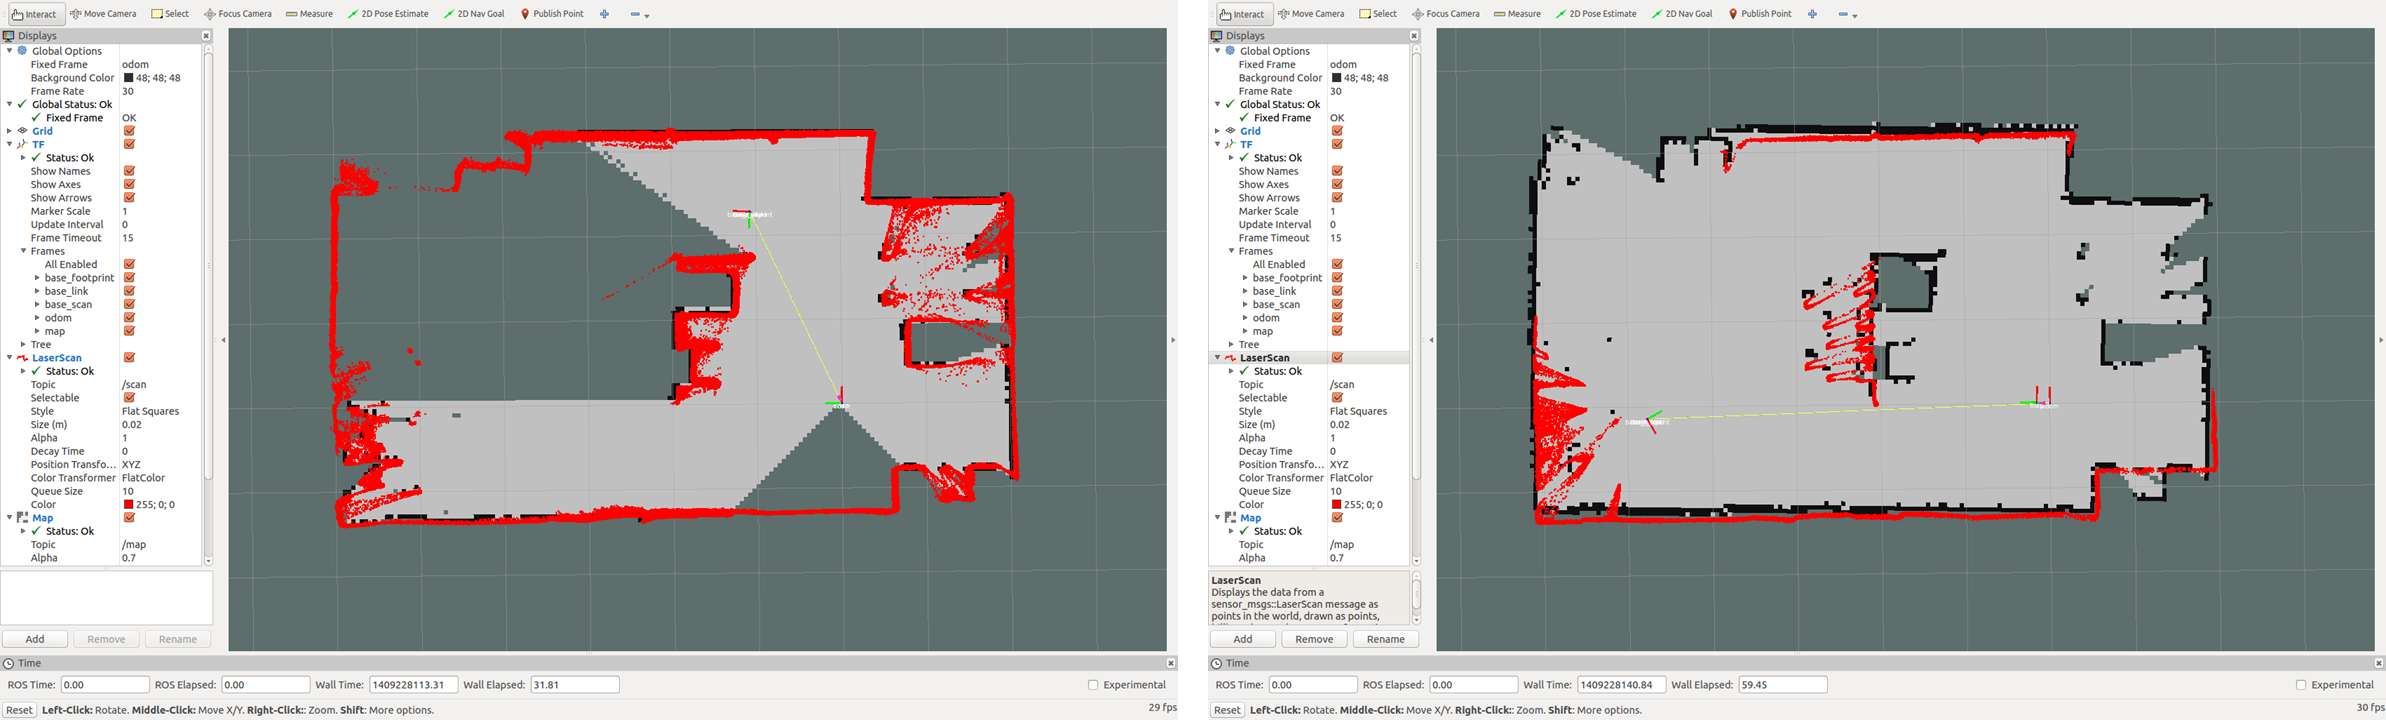
\includegraphics[width=12cm]{pictures/chapter10/pic_10_06.png}
  \caption{環境地図作成の様子}
\end{figure}

\begin{figure}[htp]
  \centering
  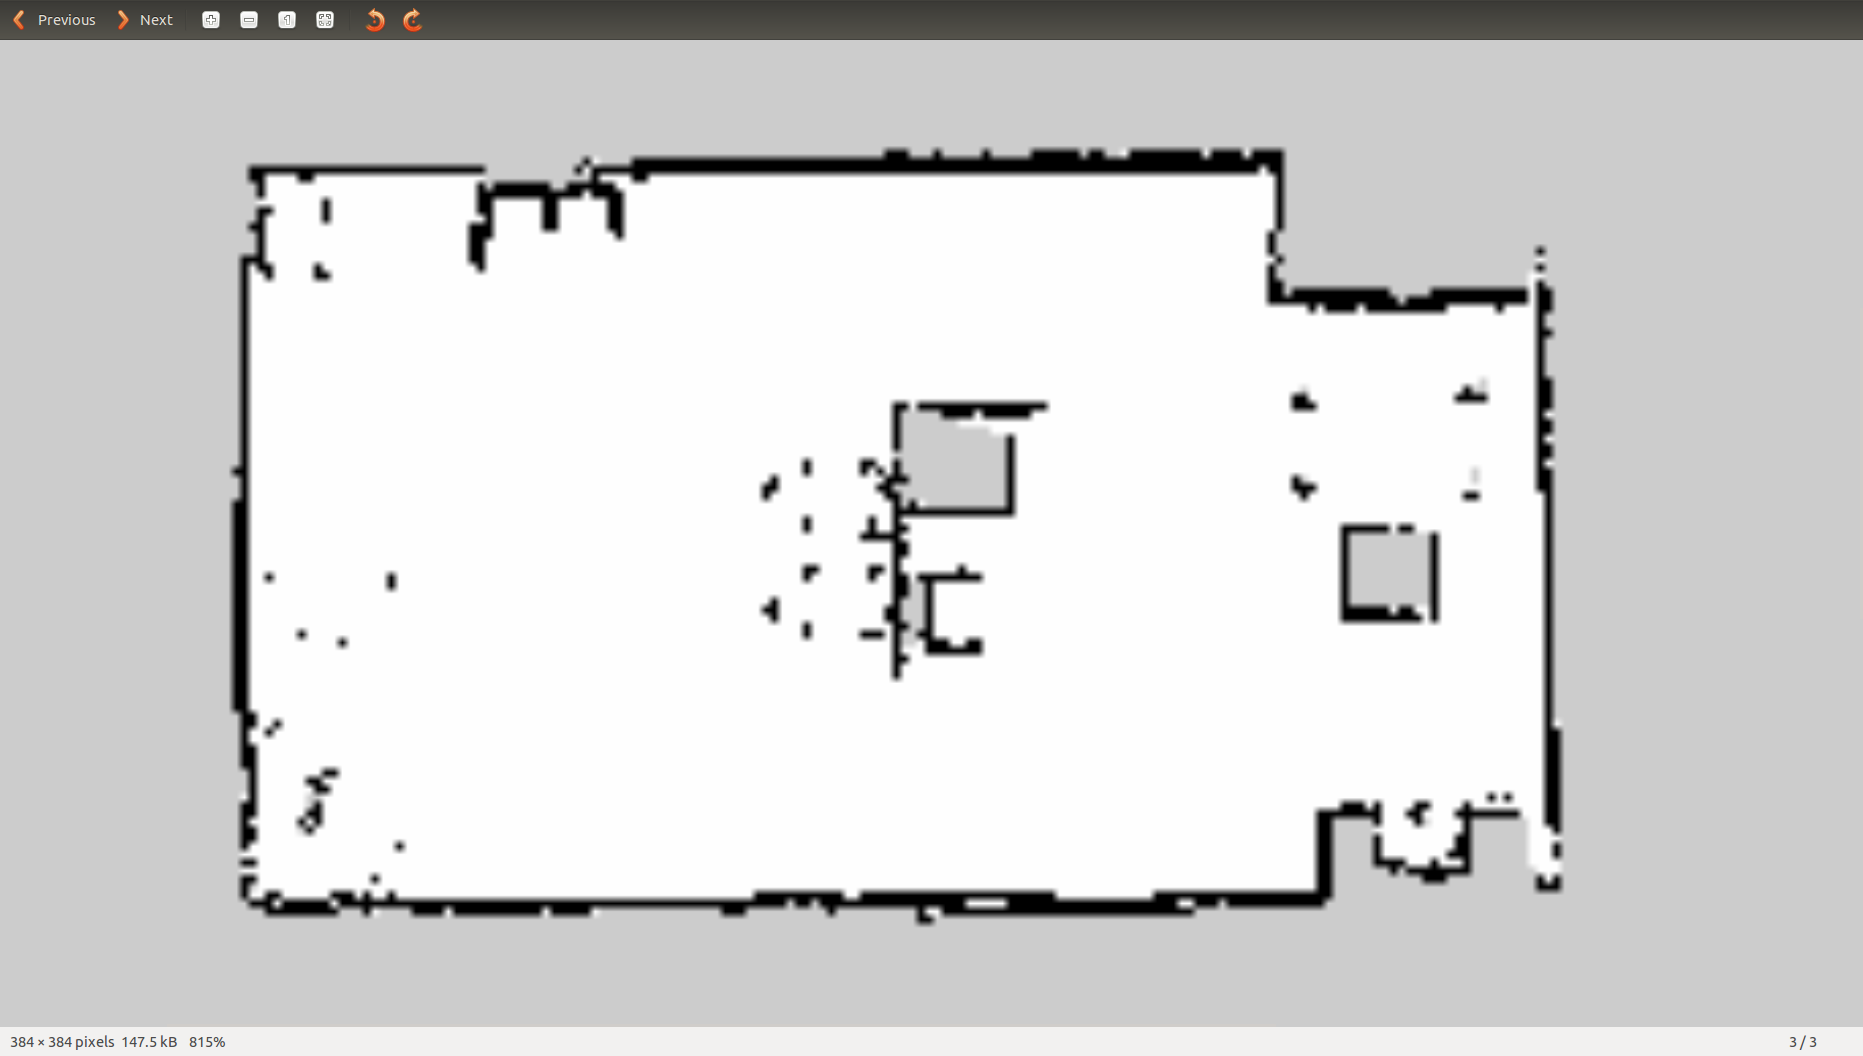
\includegraphics[width=10cm]{pictures/chapter10/pic_10_07.png}
  \caption{完成した環境地図}
\end{figure}

%-------------------------------------------------------------------------------
\subsection{保存したbagファイルを利用したSLAM}

ここでは、KobukiやLRFを実際に動作させなくても、SLAMが再現できることを確認する。以降では前節で保存しておいたbagファイルを使用するが、実機がなくbagファイルが生成できない場合でも、必要なファイルを以下のアドレスからダウンロードできる。ダウンロードしたファイルは圧縮されているので、rosbag decompressコマンドで解凍した後、適当なフォルダに保存する。

\begin{lstlisting}[language=ROS]
$ wget https://github.com/irvs/rosbook_kobuki/raw/master/kobuki_slam/scan_data.bag
$ rosbag decompress scan_data.bag
\end{lstlisting}

以降は、前節で説明したSLAMの実行方法と同じである。ただしrosbagを保存 (record)ではなく、再生 (play)する。これにより、SLAMを実行しているときと同じトピックが配信される。ただし、シミュレーション時刻のパラメータである「use\_sim\_time」を有効にして、実際の時刻ではなく、保存したトピックの時刻を使うように設定する必要がある。

\begin{lstlisting}[language=ROS]
$ roscore
$ rosparam set use_sim_time true
$ roslaunch kobuki_slam kobuki_slam_demo.launch
$ rosrun rviz rviz -d `rospack find kobuki_slam`/rviz/kobuki_slam.rviz
$ rosbag play ./scan_data.bag
$ rosrun map_server map_saver
\end{lstlisting}

%-------------------------------------------------------------------------------
\section{ROSを用いたSLAMの詳細}\index{ROSを用いたSLAMの詳細}

本節では、SLAMで使用されるROSパッケージについて、作成法と設定法を解説し、ROSによるSLAMの実現手法について解説する。読み進めるには、kobukiメタパッケージ、slam\_gmappigメタパッケージに含まれるgmappingパッケージ、navigationメタパッケージに含まれるmap\_serverパッケージの動作については理解しておく必要がある。これには10.2節を参照してほしい。SLAMで用いられる要素技術の解説は10.4節で行う。

%-------------------------------------------------------------------------------
\subsection{占有格子地図}

本項では、環境地図としてROSコミュニティで一般的に広く使用されている2次元の占有格子地図 (Occupancy Grid Map)について説明する  。10.2.4項  で得られた環境地図も占有格子地図である。一例を図10-8に示す。白い領域は、ロボットが移動可能な自由空間 (free area)、黒い領域は移動不可能な占有空間 (occupied area)、灰色はセンサ情報が得られて  いない未知空間 (unknown area)を表す。

\begin{figure}[htp]
  \centering
  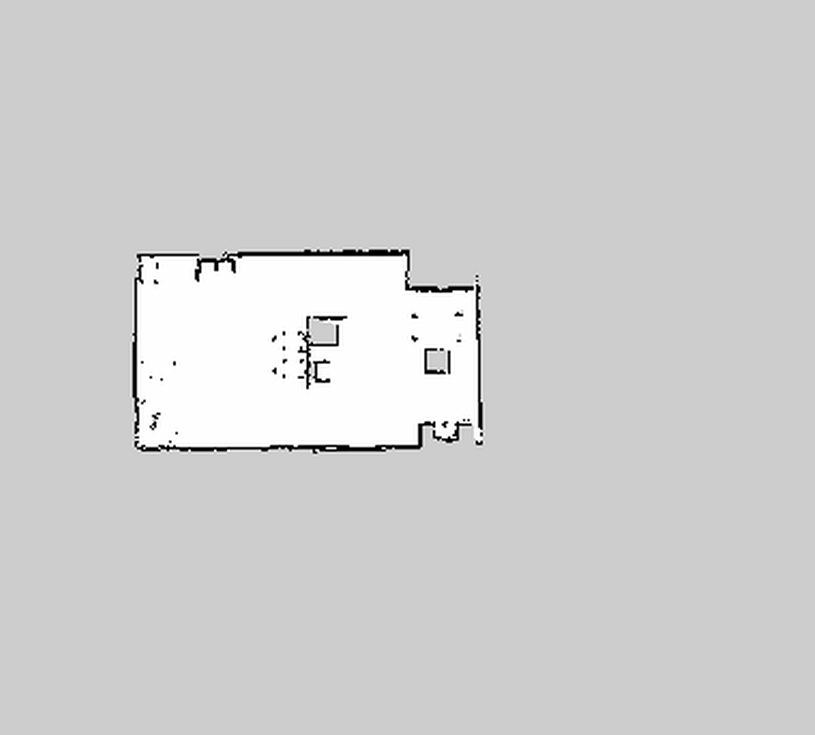
\includegraphics[width=10cm]{pictures/chapter10/pic_10_08.png}
  \caption{完成した占有格子地図}
\end{figure}

占有格子地図  は、0から255までの濃淡値で表される。この値は、占有状態を表現した占有確率を表し、ベイズの定理に基づき観測の事後確率として求められる。  占有確率occは occ = (255 - color\_avg) / 255と表現される。color\_avgは8bitで、画像が24bit画像であれば color\_avg = (セルのグレースケール値 / 0xFFFFFF × 255) となる。このoccが1に近くなるほど占有されている確率が高くなり、0に近いほど占有されていない確率が高いことを意味する。
ROSのメッセージ (nav\_msgs/OccupancyGrid)で環境地図の情報が配信されるときは、占有確率を整数-1および[0〜100]に変換している。「0」に近いほど占有確率が低く、移動できる可能性の高い自由空間、「100」に近いほど占有確率が高く、移動できる可能の低い占有空間であり  、また「-1」を未知空間と定義している。
前述のmap\_serverノードでは、環境地図をportable graymap format形式のファイル*.pgmで保存する。また、*.yamlファイルも同時に保存しており、ここに環境地図の情報が記載されている。例えば、10.2節で作成した環境地図の情報(map.yaml)を確認すると、以下のように表示される。

\begin{lstlisting}[language=ROS]
image: map.pgm
resolution: 0.050000
origin: [-10.000000, -10.000000, 0.000000]
negate: 0
occupied_thresh: 0.65
free_thresh: 0.196
\end{lstlisting}

imageは環境地図のファイル名、resolutionは環境地図の解像度であり、ここでは解像度が0.05m/pixelである。originの3つの数値は、環境地図の左下の画素に対応する実際の空間のx、y座標  とz軸回りの回転角度yawを表し、ここではx = -10m、y = -10mである。 negateが1のとき、占有空間と自由空間の値が反転している。  また、occupied\_threshは閾値であり、占有確率がこの値を超えると移動不可能な占有空間、超えないと移動可能な自由空間と見なされる。

%-------------------------------------------------------------------------------
\subsection{SLAMに必要な情報}

SLAMに必要な情報は、「距離センサから得られる距離情報」と「距離センサの位置情報」である。
まず、距離センサから得られる距離情報とは、LRF、デプスカメラなどの距離センサを用いて、XY平面に平行な面内で得られた対象物までの距離値  である。
次に、距離センサの位置情報について考える。距離センサは移動ロボットに固定されているが、単純にロボットの座標値をセンサの座標値として扱うことはできない。オドメトリ情報であるロボットの現在位置に、距離センサの取り付け位置の情報を加えた値が距離センサの位置情報となる。
通常、距離センサから得られる距離情報はscanトピック、オドメトリ情報やセンサ取り付け位置などの座標変換情報はtfトピックで表される。図10-9のように、scanトピックとtfトピックの2つの情報に基づいてSLAMを実行し、環境地図であるmapトピックを生成する。

\begin{figure}[htp]
  \centering
  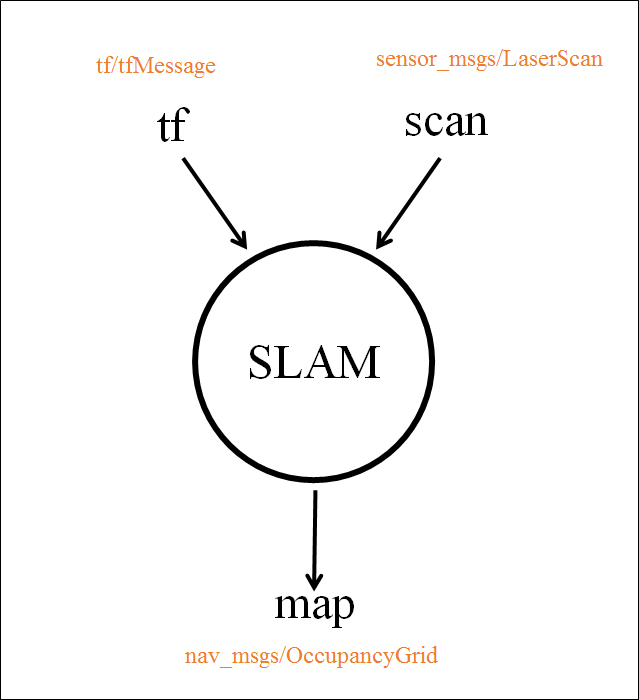
\includegraphics[width=10cm]{pictures/chapter10/pic_10_09.png}
  \caption{tfトピックとscanトピック、mapトピックの関係}
\end{figure}

%-------------------------------------------------------------------------------
\subsection{kobuki\_slamの機能と処理}

前節では、Kobukiを用いてSLAMを実行するために、kobukiノードに加えてkobu\\ki\_slamパッケージを利用した。このパッケージには、SLAMの実行に必要なノードをまとめたkobuki\_slam.launch ファイルが含まれている。図10-10に、このlaunchファイルで起動されるノードとトピックの流れを示す。

\begin{figure}[htp]
  \centering
  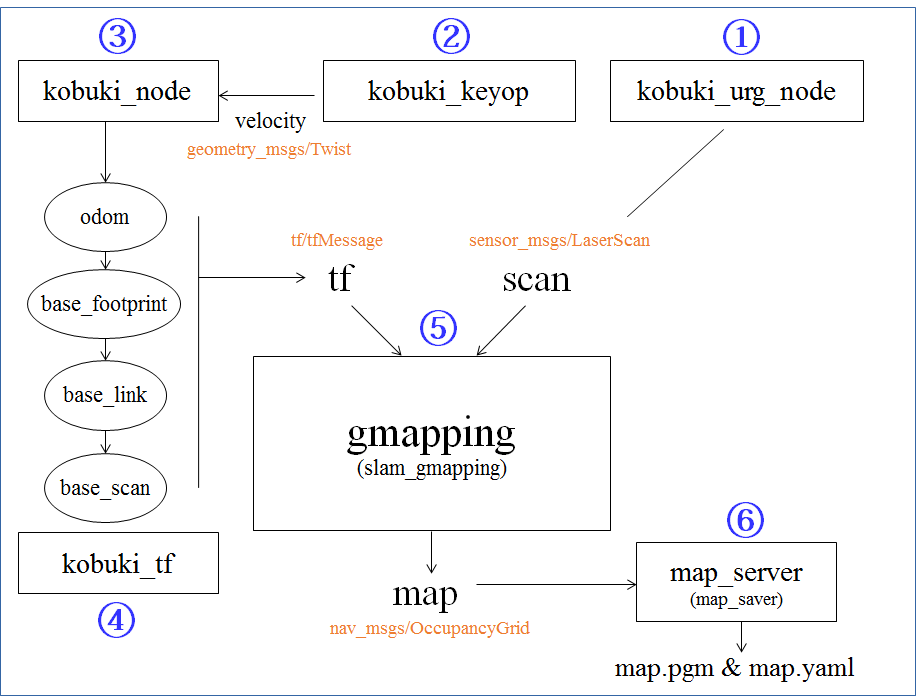
\includegraphics[width=12cm]{pictures/chapter10/pic_10_10.png}
  \caption{kobuki\_slam.launchファイルで実行されるノードとトピック}
\end{figure}

図10-10で\circled{1}~\circled{6}の番号をつけたノードについて、それぞれ説明する。

\setcounter{num}{0}

\stepcounter{num}\circled{\thenum} kobuki\_urg\_node

LRFのセンサドライバーノードを実行して、SLAMに必要なscanトピックをslam\_\\gmappingノードに配信する。

\stepcounter{num}\circled{\thenum} kobuki\_keyop

キーボード入力値を受け取り、Kobukiノードに並進速度と回転速度の指令値を配信する。

\stepcounter{num}\circled{\thenum} kobuki\_node

Kobukiノードは、ユーザーからの指令を受けて、実際にロボットを移動させるノードである。このとき、Kobukiのオドメトリ基準点 (Kobukiでは左右車輪の中央)の位置座標odomを配信すると同時に、座標変換情報であるtfトピック  も配信する。また、ロボット本体の基準点の床面投影点である  base\_footprintもtfトピックで配信する。

\stepcounter{num}\circled{\thenum} kobuki\_tf

センサの位置座標であるbase\_scanをtfトピックとしてSLAMに渡すために、odom → base\_footprint → base\_link → base\_scanの座標変換を配信する。ここで、base\_linkとはロボット本体の基準点であり、base\_scanは距離センサのロボット本体への取り付け位置である。

\stepcounter{num}\circled{\thenum} slam\_gmapping

距離センサから得られたscanトピックとセンサの位置情報であるtfトピックを用いて、環境地図を作成する。

\stepcounter{num}\circled{\thenum} map\_saver

環境地図の情報であるmap.pgm、map.yamlファイルを生成する。このノードはmap\_serverパッケージに含まれる。

%-------------------------------------------------------------------------------
\subsection{ロボットの各部分の相対座標変換 (tf)}

図10-11は、「rosrun rqt\_tf\_tree rqt\_tf\_tree」コマンドで確認できるtf注4のtreeビューアで、ロボットとセンサ間の座標変換情報を示している。
10.3.1で説明したように、距離センサの位置情報は、オドメトリ情報であるロボットの現在位置に、距離センサの取り付け位置の情報を加えた値である。実際に図10-11より、odom → base\_footprint → base\_link → base\_scanの順に位置情報が関連付けられていることがわかる。SLAMを行うには、このすべてのtf情報 (tfトピックとして配信される座標変換情報)が  必要である。

\begin{figure}[htp]
  \centering
  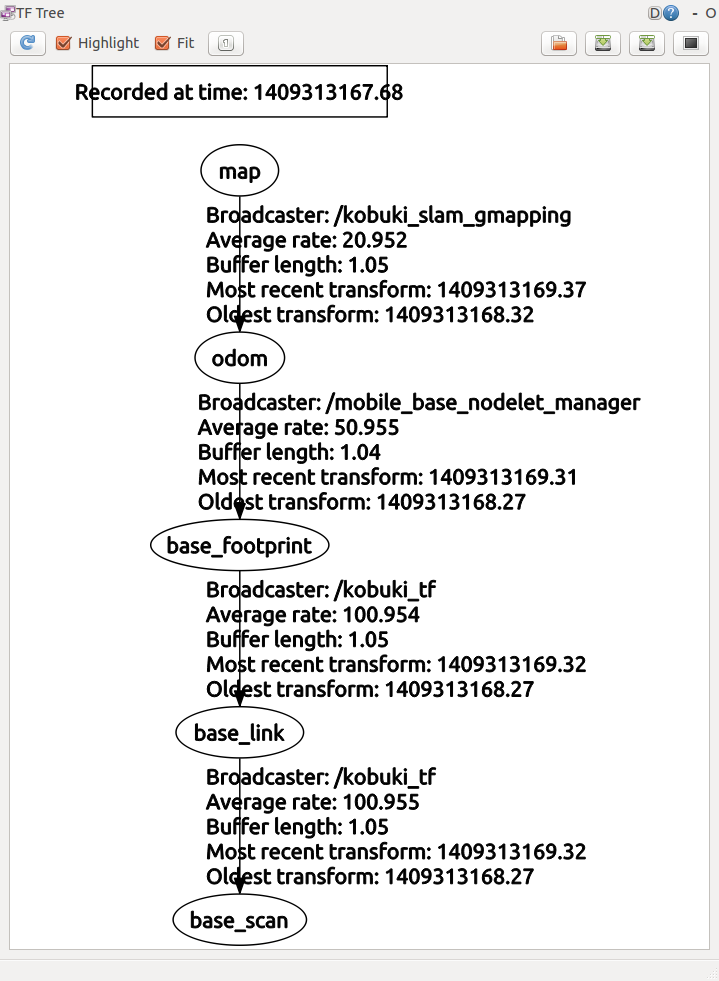
\includegraphics[width=10cm]{pictures/chapter10/pic_10_11.png}
  \caption{ロボット各部の座標変換情報}
\end{figure}

%-------------------------------------------------------------------------------
\subsection{kobuki\_tfパッケージの作成}

ここでは、tf情報を用いた座標変換の仕組みを理解するために、kobuki\_tfパッケージを自作してみよう。rosbook\_kobukiリポジトリをすべてダウンロードした場合には、kobuki\_tfパッケージが既に存在しているので、あらかじめ「rm –r ~/catkin\_ws/src/kobuki\_tf」などによりこれを削除しておく。

\begin{lstlisting}[language=ROS]
$ rm -r ~/catkin_ws/src/kobuki_tf
\end{lstlisting}

次に、以下のコマンドで新たにkobuki\_tfパッケージを生成し、エディタでsrcディレクトリのtf\_broadcaster.cppファイルを新規に開き、以下の内容をコピーする。

\begin{lstlisting}[language=ROS]
$ cd ~/catkin_ws/src/
$ catkin_create_pkg kobuki_tf roscpp tf geometry_msgs
$ gedit kobuki_tf/src/tf_broadcaster.cpp
\end{lstlisting}

\textbf{ファイル名: tf\_broadcaster.cpp}

\begin{lstlisting}[language=C++]
#include <ros/ros.h>
#include <tf/transform_broadcaster.h>

int main(int argc, char** argv){
  ros::init(argc, argv, "kobuki_tf");
  ros::NodeHandle n;
  ros::Rate r(100);
  tf::TransformBroadcaster broadcaster;

  while(n.ok()){
    broadcaster.sendTransform(
    tf::StampedTransform(
      tf::Transform(
        tf::Quaternion(0, 0, 0, 1),
        tf::Vector3(0.0, 0.0, 0.01)),
        ros::Time::now(), "base_footprint", "base_link"));
    broadcaster.sendTransform(
      tf::StampedTransform(
        tf::Transform(
          tf::Quaternion(0, 0, 0, 1),
          tf::Vector3(0.0, 0.0, 0.24)),
          ros::Time::now(), "base_link", "base_scan"));
    r.sleep();
  }
}
\end{lstlisting}

既にkobuki\_nodeでは、odom → base\_footprintのtfが提供されている。本ノードはセンサデータを座標変換するため、これらに加えてbase\_linkとbase\_scanをtfトピックとして配信する。これにより、以下のすべての座標変換が可能となる。

odom → base\_footprint → base\_link → base\_scan

tf\_broadcaster.cppファイルでは、base\_linkは床 (またはbase\_footprint)から0.01m (1cm)上に、またセンサの取り付け位置であるbase\_scanはbase\_linkから0.24m (24cm)上に設定している。
次に、CMakeLists.txtファイルを開き、次の2つの設定を追加する。

\textbf{ファイル名: CMakeLists.txt}
\begin{lstlisting}[language=make]
add_executable(kobuki_tf src/tf_broadcaster.cpp)
target_link_libraries(kobuki_tf ${catkin_LIBRARIES})
\end{lstlisting}

これによりkobuki\_tfの実行ファイルを生成できる。次のコマンドで新たに作成したkobuki\_tfパッケージ  をビルドしてみよう。

\begin{lstlisting}[language=ROS]
$ cd ~/catkin_ws && catkin_make
\end{lstlisting}

%-------------------------------------------------------------------------------
\subsection{kobuki\_slamパッケージの作成}

次に、kobuki\_slamパッケージを作成してみる。rosbook\_kobukiリポジトリをすべてダウンロードした場合には、kobuki\_slamパッケージが既に存在しているので、あらかじめ「rm –r ~/catkin\_ws/src/kobuki\_slam」などによりパッケージを削除しておく。

\begin{lstlisting}[language=ROS]
$ rm -r ~/catkin_ws/src/kobuki_slam
\end{lstlisting}

ま  ず、以下のように新たにkobuki\_slamパッケージを生成し、launchディレクトリを作成する。その後、エディタでlaunchディレクトリのkobuki\_slam.launchファイルを新規に開き、以下の内容をコピーする。

\begin{lstlisting}[language=ROS]
$ cd ~/catkin_ws/src/
$ catkin_create_pkg kobuki_slam roscpp kobuki_node urg_node
$ mkdir kobuki_slam/launch
$ gedit kobuki_slam/launch/kobuki_slam.launch
\end{lstlisting}

\textbf{ファイル名: kobuki\_slam.launch}
\begin{lstlisting}[language=XML]
<launch>
  <node pkg="urg_node" type="urg_node" name="kobuki_urg_node" output="screen">
    <param name="frame_id" value="base_scan" />
  </node>
  <node pkg="kobuki_tf" type="kobuki_tf" name="kobuki_tf" output="screen"></node>
  <node pkg="gmapping" type="slam_gmapping" name="kobuki_slam_gmapping" output="screen">
    <param name="base_frame" value="base_footprint"/>
    <param name="odom_frame" value="odom"/>
    <param name="map_update_interval" value="1.0"/>
    <param name="maxUrange" value="6.0"/>
    <param name="sigma" value="0.05"/>
    <param name="kernelSize" value="1"/>
    <param name="lstep" value="0.05"/>
    <param name="astep" value="0.05"/>
    <param name="iterations" value="5"/>
    <param name="lsigma" value="0.075"/>
    <param name="ogain" value="3.0"/>
    <param name="lskip" value="0"/>
    <param name="srr" value="0.01"/>
    <param name="srt" value="0.02"/>
    <param name="str" value="0.01"/>
    <param name="stt" value="0.02"/>
    <param name="linearUpdate" value="0.25"/>
    <param name="angularUpdate" value="0.25"/>
    <param name="temporalUpdate" value="-1.0"/>
    <param name="resampleThreshold" value="0.5"/>
    <param name="particles" value="300"/>
    <par am name="xmin" value="-10.0"/>
    <param name="ymin" value="-10.0"/>
    <param name="xmax" value="10.0"/>
    <param name="ymax" value="10.0"/>
    <param name="delta" value="0.05"/>
    <param name="llsamplerange" value="0.01"/>
    <param name="llsamplestep" value="0.01"/>
    <param name="lasamplerange" value="0.005"/>
    <param name="lasamplestep" value="0.005"/>
  </node>
</launch>
\end{lstlisting}

kobuki\_slam.launchファイルの最初の項目は、Kobukiに装着されたLRFを起動するための構文である。paramオプションによりframe\_idパラメータをbase\_scanに変更している。

\subsubsection{kobuki\_urg\_node ノード設定}

\begin{lstlisting}[language=XML]
  <node pkg="urg_node" type="urg_node" name="kobuki_urg_node" output="screen">
    <param name="frame_id" value="base_scan" />
  </node>
\end{lstlisting}

次は、このlaunchファイルの実行時に、前項で作成したkobuki\_tfも同時に起動するための構文である。

\subsubsection{kobuki\_tfノード設定}

\begin{lstlisting}[language=XML]
<node pkg="kobuki_tf" type="kobuki_tf" name="kobuki_tf" output="screen"> </node>
\end{lstlisting}

次は、slam\_gmappingを実行する際に必要なさまざまなオプションを、使用するロボットとセンサに合わせて変更している。

\subsubsection{slam\_gmappingノード設定}

\begin{lstlisting}[language=XML]
<param name = "base_frame" value = "base_footprint" />  %*ロボットの基本フレーム*)
<param name = "odom_frame" value = "odom" />      %*オドメトリフレーム*)
<param name = "map_update_interval" value = "1.0" />    %*環境地図の更新間隔 (sec)*)
<param name = "maxUrange" value = "6.0" />  %*レーザー最大到達距離 (meter)*)
<param name = "sigma" value = "0.05" />   %*レーザー対応探索の標準偏差*)
<param name = "kernelSize" value = "1" />  %*レーザー対応探索のウィンドウサイズ*)
<param name = "lstep" value = "0.05" />   %*初期探索ステップ (移動)*)
<param name = "astep" value = "0.05" />   %*初期探索ステップ (回転)*)
<param name = "iterations" value = "5" /> %*スキャンマッチングの繰り返し回数*)
<param name = "lsigma" value = "0.075" /> %*ビーム尤度計算の標準偏差*)
<param name = "ogain" value = "3.0" />    %*尤度平滑化ゲイン*)
<param name = "lskip" value = "0" />    %*スキャンマッチングを行う間隔*)
<param name = "srr" value = "0.01" />   %*オドメトリエラー (移動→移動)*)
<param name = "srt" value = "0.02" />   %*オドメトリエラー (移動→回転)*)
<param name = "str" value = "0.01" />   %*オドメトリエラー (回転→移動)*)
<param name = "stt" value = "0.02" />   %*オドメトリエラー (回転→回転)*)
<param name = "linearUpdate" value = "0.25" />  %*処理開始に必要な最低移動距離*)
<param name = "angularUpdate" value = "0.25" /> %*処理開始に必要な最低回転角度*)
<param name = "temporalUpdate" value = " - 1.0" />  %*最後にスキャンを行った時間がこの更新時*)
%*間を過ぎた場合、スキャンを行う。この値が0以下の場合は使用しない。*)
<param name = "resampleThreshold" value = "0.5" />  %*リサンプルを行う閾値*)
<param name = "particles" value = "300" />    %*パーティクル数*)
<param name = "xmin" value = " - 10.0" />  %* 最小のx座標*)
<param name = "ymin" value = " - 10.0" />   %*最小のy座標*)
<param name = "xmax" value = "10.0" />      %*最大のx座標*)
<param name = "ymax" value = "10.0" />      %*最大のy座標*)
<param name = "delta" value = "0.05" />     %*環境地図の解像度: 長さ/ピクセル*)
<param name = "llsamplerange" value = "0.01" /> %*尤度計算の範囲 (移動)*)
<param name = "llsamplestep" value = "0.01" />  %*尤度計算のステップ幅 (移動)*)
<param name = "lasamplerange" value = "0.005" />  %*尤度計算の範囲 (回転)*)
<param name = "lasamplestep" value = "0.005" /> %*尤度計算のステップ幅 (回転)*)
\end{lstlisting}

以上でSLAMによる環境地図の作成に必要な事項を説明した。次節では、SLAMで用いられる要素技術について解説する。

%-------------------------------------------------------------------------------
\section{SLAMの要素技術}\index{SLAMの要素技術}

%-------------------------------------------------------------------------------
\subsection{センサとアルゴリズム}

SLAMは位置推定と環境地図の作成を同時に行う手法である。位置推定に使用される代表的なセンサ  には、エンコーダと慣性センサ (IMU、Inertial Measurement Unit)がある。エンコーダは、駆動部である車輪の回転量を測定し、ロボットの位置や姿勢を計算するオドメトリ法で用いられる。車輪の滑りや高低差などにより大きな誤差が生じるが、同時に慣性センサで速度や加速度を測定することで、位置情報の補正が可能である。エンコーダを用いず、慣性センサだけで位置を推定する場合もある。
SLAMでは、これらのセンサから得られた位置推定値は、距離センサやカメラにより得られた周辺環境の情報に基づいて、再び補正される。補正された位置の推定  には、カルマンフィルタ、マルコフ位置推定、パーティクルフィルタを利用したモンテカルロ位置推定などが用いられる。
環境地図の作成によく用いられるセンサ  は、LRF、超音波センサ、赤外線距離センサ、LiDAR、レーダーなどの距離センサである。近年では、デプスカメラ (Kinect、Xtionなど)が普及し、これらを利用したSLAMも開発されている。

%-------------------------------------------------------------------------------
\subsection{周囲環境の情報に基づく位置推定法}

ロボットの位置推定が正確であれば、その位置を基準に得られた周囲環境の情報から環境地図が作成できるが、計測誤差のために位置情報は不正確である。そこで、周囲環境の情報を用いて位置推定値を補正し、位置推定の信頼性、精度を向上するための様々な位置推定法が提案されている。本項では、その代表例として、カルマンフィルタ、パーティクルフィルタについて解説する。

\subsubsection{カルマンフィルタ (Kalman filter)}

位置推定では、Rudolf E. Kalmanが開発したカルマンフィルタが多く使用されている。カルマンフィルタは、正規分布に従うノイズ (ガウスノイズ)を含む線形システムに対し、ベイズの定理 に基づいて対象の状態を最尤推定する再帰フィルタである 。図10-12の処理の流れを示す。まずシステムの動作モデル  (例えばオドメトリ法や等速直線モデル)に基づいて、現時刻のシステムの状態を予測する。次に、より正確な状態量を推定するために、この予測値と実際の計測値との間の誤差を用いてシステムの状態を補正する。この補正に、これまでに得られた誤差の統計量を利用する ことで、予測値と計測値を確率的に最適に融合する。これを繰り返し実行することで、推定位置精度が向上する。
カルマンフィルタを利用したSLAMでは、ある時刻までに得られている環境地図と自己位置の推定値から、次時刻で観測されるべき周囲環境を予測し、これと実際に観測された周囲環境との差を誤差として用いる。この誤差をもとに自己位置を補正することで、自己位置と環境地図の推定精度を同時に向上する。

\begin{figure}[htp]
  \centering
  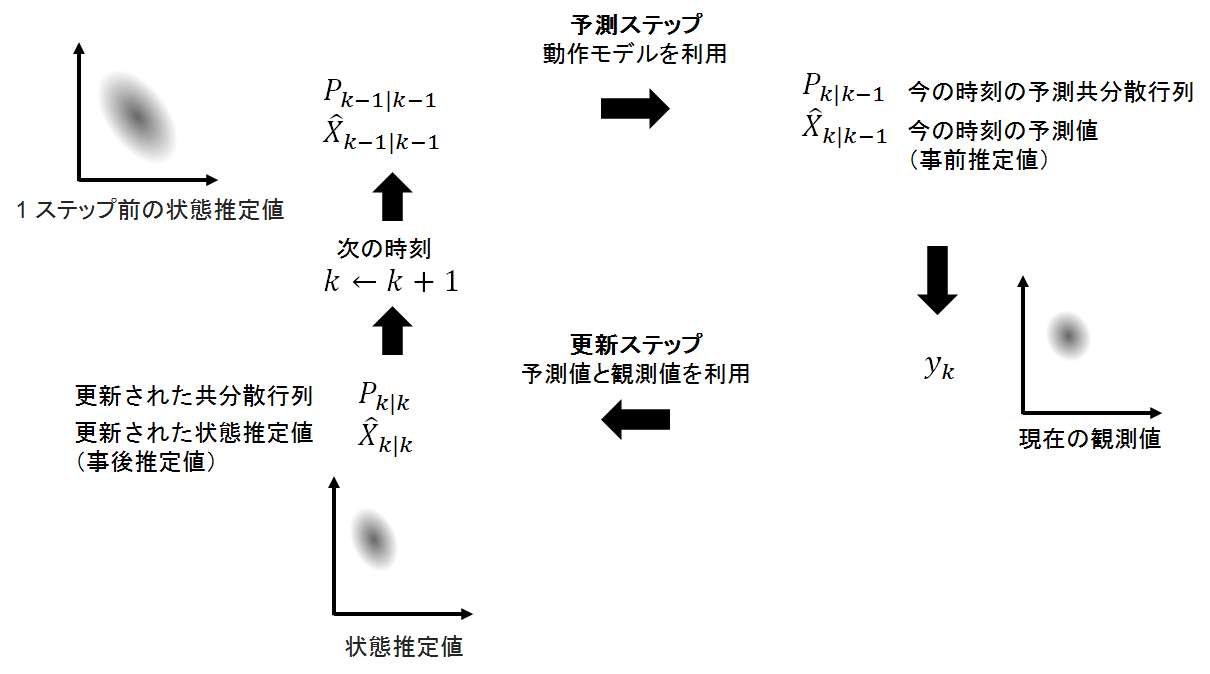
\includegraphics[width=\columnwidth]{pictures/chapter10/pic_10_12.png}
  \caption{カルマンフィルタの処理の流れ}
\end{figure}

ロボットやセンサは非線形システムである場合が多いが、カルマンフィルタは線形システムを仮定している。したがって、ロボットやセンサのような非線形システムにカルマンフィルタを適用するには、工夫が必要になる。 非線形システムを局所的に線形化してカルマンフィルタを適用する拡張カルマンフィルタ (EKF、Extended Kalman Filter)はその一例であり、実際に広く利用されている。カルマンフィルタにはこの他にも多くのバリエーションがあり、ノイズにガウス性を仮定しない アンセンテッドカルマンフィルタ (UKF、Unscented Kalman Filter)   などが提案されている。また、他のアルゴリズムと組み合わせて使用されることもあり、例えば、パーティクルフィルタ (後述)と組み合わせたRBPF (Rao-Blackwellized Particle Filter)はSLAMで広く用いられている。


\subsubsection{パーティクルフィルタ (Particle filter)}

カルマンフィルタは、線形システムとガウスノイズが仮定できる場合は最適なフィルタであるが、それ以外のシステムでは性能が低下する。一方、現実世界のほとんどは非線形システムである。そこで、非線形なシステムに適用可能な手法として、パーティクルフィルタを紹介する。
パーティクルフィルタは、近年、物体追跡や状態推定で盛んに利用されている手法である。 パーティクルフィルタは、多数の状態候補から  の再サンプリングにより、システム  の状態を推定する。すなわち、システムの状態候補 (サンプル)を多数用意し、その中から観測結果と矛盾しない状態を再サンプリングする。これを多数回繰り返すことで、観測に最適なサンプルを抽出する方法である。  このサンプルをパーティクル (粒子)として表現することから、パーティクルフィルタ (あるいは逐次モンテカルロ法 (Sequential Monte Carlo)と呼ばれる。
パーティクルフィルタをロボットの位置同定に適用した手法にモンテカルロ位置推定 (Monte Carlo Localization)がある。移動ロボットの場合、パーティクルが保持する状態量は、位置 (x、y)と姿勢 (θ)、重み (weight)である。重みは、パーティクルの保持する状態量と実際の計測値との一致度に基づいて計算され、重みの大きさに応じてパーティクルが再サンプリングされる確率を変更する。
このパーティクルフィルタは、次の5つの処理からなる。①初期化の後、②〜⑤を繰り返し実行しながら、ロボットの推定位置の確率分布を計算する。

\setcounter{num}{0}

\stepcounter{num}\circled{\thenum} 初期化
ロボットの位置姿勢が全くわからないときは、N個  のパーティクルを、位置姿勢が取り得る範囲内にランダムに配置する。初期パーティクルの重みはそれぞれ1/Nとする。Nは経験的に決定し、通常は数百個である。初期位置が既知である場合には、その近傍にパーティクルを配置する。

\stepcounter{num}\circled{\thenum} 予測
ロボットの動作モデルに基づき、オドメトリ情報などの観測された移動量にノイズを加えて、各パーティクルを遷移させる。

\stepcounter{num}\circled{\thenum} 更新
LRFなどからの観測情報とパーティクルの状態量を基に、観測情報と状態量の一致度を計算し、各パーティクルの重みを更新する。

\stepcounter{num}\circled{\thenum} 位置推定
すべてのパーティクルの位置姿勢と重みを用いて、重み付き平均値や中央値、最大の重みをもつパーティクルの値などにより、ロボットの推定位置を計算する。

\stepcounter{num}\circled{\thenum} 再サンプリング
重みに比例した確率で、パーティクルを再サンプリングする。すなわち、重みが小さいパーティクルよりも、重みが大きいパーティクルを優先的に選択する。選択されないパーティクルは消去される。

なお、パーティクルフィルタにより正確な状態量の推定を行うには、サンプル数が十分でなければならない。上記では推定する状態量は位置・姿勢の3つであったが、SLAMではこれに加えて環境地図も推定する必要がある。しかし環境地図も状態量とすると推定すべき状態量が多くなり  、十分なサンプル数を用意するのが非現実的になる。そこでパーティクルフィルタとカルマンフィルタを同時に使用することでパーティクルフィルタの推定状態量を低減するRBPFを用いたSLAMも提案されている。

\begin{exercise}[パーティクルフィルタの解説書]
  パーティクルフィルタなど、ロボット分野で話題の確率的手法については、「Probabilistic Robotics」   (2005年、Sebastian Thrun, Wolfram Burgard, Dieter Fox著、The MIT Press)を一読することを推奨する。ユダシティのオンライン講座「Artificial Intelligence for Robotics」も参考にしてほしい。\\
  ユダシティオンライン講座 https://www.udacity.com/course/cs373
\end{exercise}

以上で、ROSでのSLAMの利用についての説明を終える。gmappingのより詳しい説明は、以下のコラム内の参考論文を参照してほしい。次節では、ナビゲーションについて解説する。

\begin{exercise}[OpenSLAMとGmapping]
  SLAMは、近年盛んに研究されている。SLAMに関する有益な最新情報は、学術誌や学会発表を通じて得ることができる。また、多くのアルゴリズムがオープンソースとして公開されている。代表的な手法を集めたOpenSLAM.orgというサイトもあり、まずはこちらを参照するとよい。10.4節で使用したgmapping注5もこのサイトで紹介されているが、ROSコミュニティでは頻繁に使用されている。GmappingはグリッドベースのFastSLAM2.0の実装である。Gmappingについては、以下の論文を参照してほしい。
  Grisetti, Giorgio, Cyrill Stachniss, and Wolfram Burgard, Improving grid-based slam with rao-blackwellized particle filters by adaptive proposals and selective resampling, Proceedings of the 2005 IEEE International Conference on Robotics and Automation, pp. 2432-2437, 2005.
  Grisetti, Giorgio, Cyrill Stachniss, and Wolfram Burgard, Improved techniques for grid mapping with rao-blackwellized particle filters, IEEE Transactions on Robotics, Vol.23, No.1, pp.34-46, 2007
\end{exercise}

%-------------------------------------------------------------------------------
\section{ROSを用いたナビゲーションの実行手順}\index{ROSを用いたナビゲーションの実行手順}

本節ではROSを用いたナビゲーションについて解説する。ナビゲーションで用いられる要素技術については10.7節で紹介する。ナビゲーションのためのロボットのハードウェアとして、10.2節と同様に、移動ロボットにはKobukiを、センサにはLRFを用いる。計測環境もSLAMを実行した環境と同様である。本節では、SLAMで作成した環境地図を利用して、定められた目的地までロボットを移動させるナビゲーションについて説明する。ただし、実行方法のみを記述し、各パッケージの説明は次節で詳しく行う。

%-------------------------------------------------------------------------------
\subsection{ナビゲーションのためのROSパッケージ}

この節で使用するナビゲーション関連のROSパッケージは、kobukiメタパッケージと、SLAMの項で作成したkobuki\_tfパッケージ、navigationメタパッケージのmove\_base、amcl、map\_serverパッケージなどである。まず、すべてのパッケージをインストールする。 な お、本節で用いるすべてのパッケージは、Kobuki本体に接続されたノートパソコンにインストールする必要がある。また、ノード、launchファイルは、すべてKobuki本体に接続されたノートパソコンで実行しなくてはならない。ただし、RVizおよびその他の視覚化ツールに関しては、デスクトップ上で実行しても構わない。
以下は、ナビゲーション関連のROSパッケージをインストールするためのコマンドである。

\begin{lstlisting}[language=ROS]
$ sudo apt-get install ros-indigo-kobuki*
$ sudo apt-get install ros-indigo-navigation
\end{lstlisting}

センサパッケージは、使用するセンサに合わせて関連のパッケージをインストールする。本節では、前節のSLAMと同様にLRFを用いる。北陽電機製LRF (URG-04LXとUTM-30LXシリーズ)センサパッケージのインストールは、次の通りである。

\begin{lstlisting}[language=ROS]
$ sudo apt-get install ros-indigo-urg-node
\end{lstlisting}

%-------------------------------------------------------------------------------
\subsection{ナビゲーションの実行}

前項で示したパッケージのインストールを終えたら、  次の手順でナビゲーションを実行する。

\setcounter{num}{0}

\stepcounter{num}\circled{\thenum} 関連パッケージのダウンロードとビルド

10.2.4項で関連パッケージををダウンロードしていない場合には、  次のGithubアドレスから関連パッケージをダウンロードして  ビルドする。

\begin{lstlisting}[language=ROS]
$ cd ~/catkin_ws/src
$ git clone https://github.com/irvs/rosbook_kobuki.git
$ cd ~/catkin_ws && catkin_make
\end{lstlisting}

\stepcounter{num}\circled{\thenum} Kobukiノードの実行

roscoreを実行した後、新しいターミナルウィンドウを二つ開き、roscoreおよびKobukiノードを実行する。

\begin{lstlisting}[language=ROS]
$ roscore
\end{lstlisting}

\begin{lstlisting}[language=ROS]
$ roslaunch kobuki_node minimal.launch --screen
\end{lstlisting}

\stepcounter{num}\circled{\thenum} kobuki\_navigation実行

kobuki\_navigationパッケージは、複数のlaunchファイルで構成されている。次のように、kobuki\_navigation.launchファイルを実行すると、LRFのドライバであるurg\_nodeノード、座標変換のためのkobuki\_tfノード、Kobukiの3次元モデル情報、環境地図を管理するmap\_serverノード、AMCLノード、move\_baseノードが同時に実行される。

\begin{lstlisting}[language=ROS]
$ sudo chmod a+rw /dev/ttyACM0
$ roslaunch kobuki_navigation kobuki_navigation.launch
\end{lstlisting}

以下は、kobuki\_navigation.launchの内容である。使用するロボット、センサに応じて、多くの設定値がある。ここでは、本章で使用するKobukiとLRFに合わせて設定した。このファイルを自作のロボットに適用する方法については、10.6節 で説明する。

\textbf{ファイル名: kobuki\_navigation.launch}
\begin{lstlisting}[language=XML]
<launch>
  <!-- kobuki model -->
  <arg name="urdf_file" default="$(find xacro)/xacro.py
'$(find kobuki_description)/urdf/kobuki_standalone.urdf.xacro'" />
  <param name="robot_description" command="$(arg urdf_file)" />
  <node pkg="robot_state_publisher" type="robot_state_publisher" name="robot_state_publisher" output=" screen">
    <param name="publish_frequency" type="double" value="5.0" />
  </node>

  <!-- sensor -->
  <node pkg="urg_node" type="urg_node" name="kobuki_urg_node" output="screen">
<param name="frame_id" value="base_scan" />
  </node>

  <!-- tf -->
  <node pkg="kobuki_tf" type="kobuki_tf" name="kobuki_tf" output="screen">
  </node>

  <!-- Map server -->
  <arg name="map_file" default="$(find kobuki_navigation)/maps/map.yaml"/>
  <node name="map_server" pkg="map_server" type="map_server" args="$(arg map_file)">
  </node>

  <!-- AMCL -->
  <include file="$(find kobuki_navigation)/launch/amcl.launch.xml"/>

  <!-- move_base -->
  <arg name="cmd_vel_topic" default="/mobile_base/commands/velocity" />
  <arg name="odom_topic" default="odom" />
  <node pkg="move_base" type="move_base" respawn="false" name="move_base" output="screen">
    <rosparam file="$(find kobuki_navigation)/param/costmap_common_params.yaml" command="load" ns=" global_costmap" />
    <rosparam file="$(find kobuki_navigation)/param/costmap_common_params.yaml" command="load" ns=" local_costmap" />
    <rosparam file="$(find kobuki_navigation)/param/local_costmap_params.yaml" command="load" />
    <rosparam file="$(find kobuki_navigation)/param/global_costmap_params.yaml" command="load" />
    <rosparam file="$(find kobuki_navigation)
/param/dwa_local_planner_params.yaml" command="load" />
    <rosparam file="$(find kobuki_navigation)/param/move_base_params.yaml" command="load" />
    <remap from="cmd_vel" to="$(arg cmd_vel_topic)"/>
    <remap from="odom" to="$(arg odom_topic)"/>
  </node>
</launch>
\end{lstlisting}

\stepcounter{num}\circled{\thenum} RViz実行

目的地の設定とナビゲーション結果を表示するために、プラグインをオプションに指定してRVizを起動する

\begin{lstlisting}[language=ROS]
$ rosrun rviz rviz -d `rospack find kobuki_navigation`/rviz/kobuki_nav.rviz
\end{lstlisting}

これを実行すると、図10-13のような画面が現れ、環境地図に多数の緑の矢印  が確認できる。ひとつひとつの矢印が10.4.2項で説明したパーティクルフィルタの各粒子を表している。緑の矢印の中央付近にKobukiを示す●印  がある。

\begin{figure}[htp]
  \centering
  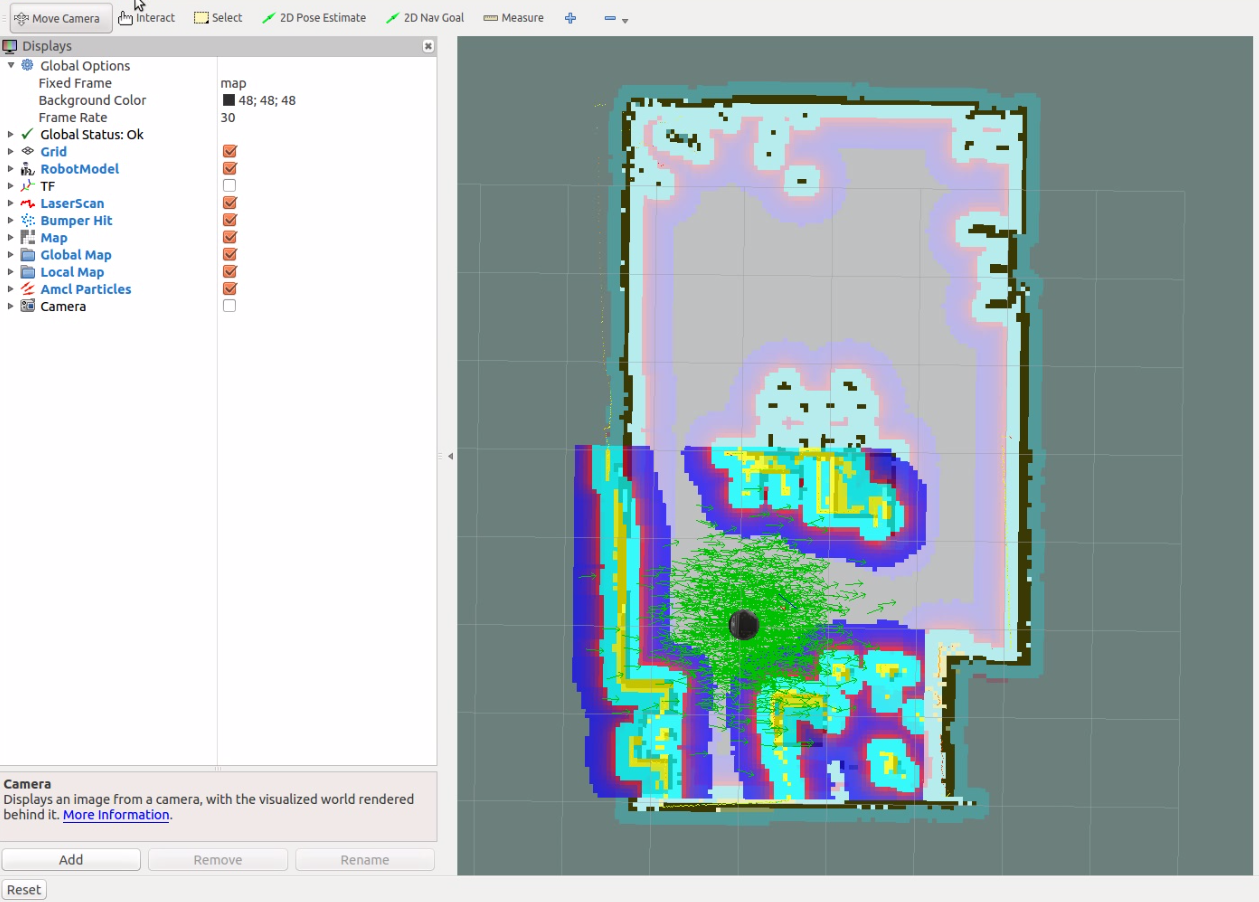
\includegraphics[width=15cm]{pictures/chapter10/pic_10_13.png}
  \caption{RVizで表示したパーティクル (ロボット周囲の矢印)}
\end{figure}

\stepcounter{num}\circled{\thenum} 初期位置・姿勢の推定

ナビゲーションの開始にあたり、 ロボットの初期位置と姿勢を指定する。RVizのメニューの[2D Pose Estimate]をクリックし、ロボットの中央をクリックすると、初期位置として大きな緑色の矢印が現れる。次にクリックしたままで、矢印がロボットの向いている方向を指すようにドラッグし、初期姿勢を指定する。   これ以降は、この緑色の矢印で指定された位置と姿勢を初期値として、ロボットの移動中の位置と姿勢 (x、y、θ)を推定していく。

\stepcounter{num}\circled{\thenum} 目的地の設定とロボットの移動

ここまで\circled{1}~\circled{5}の作業  が完了したら、ナビゲーションを実行してみよう。RVizのメニューから[2D Nav Goal]をクリックし、ロボットを移動させる目的地をクリックすると、\circled{5}と同じように  大きな緑色の矢印が現れる。次にクリックしたままで、この矢印をドラッグすることで目標姿勢を与え、目的地の位置と姿勢を設定する。その後、ロボットは作成された環境地図を用いて、目的地までの障害物を回避しながら移動する (図10-14)。

\begin{figure}[htp]
  \centering
  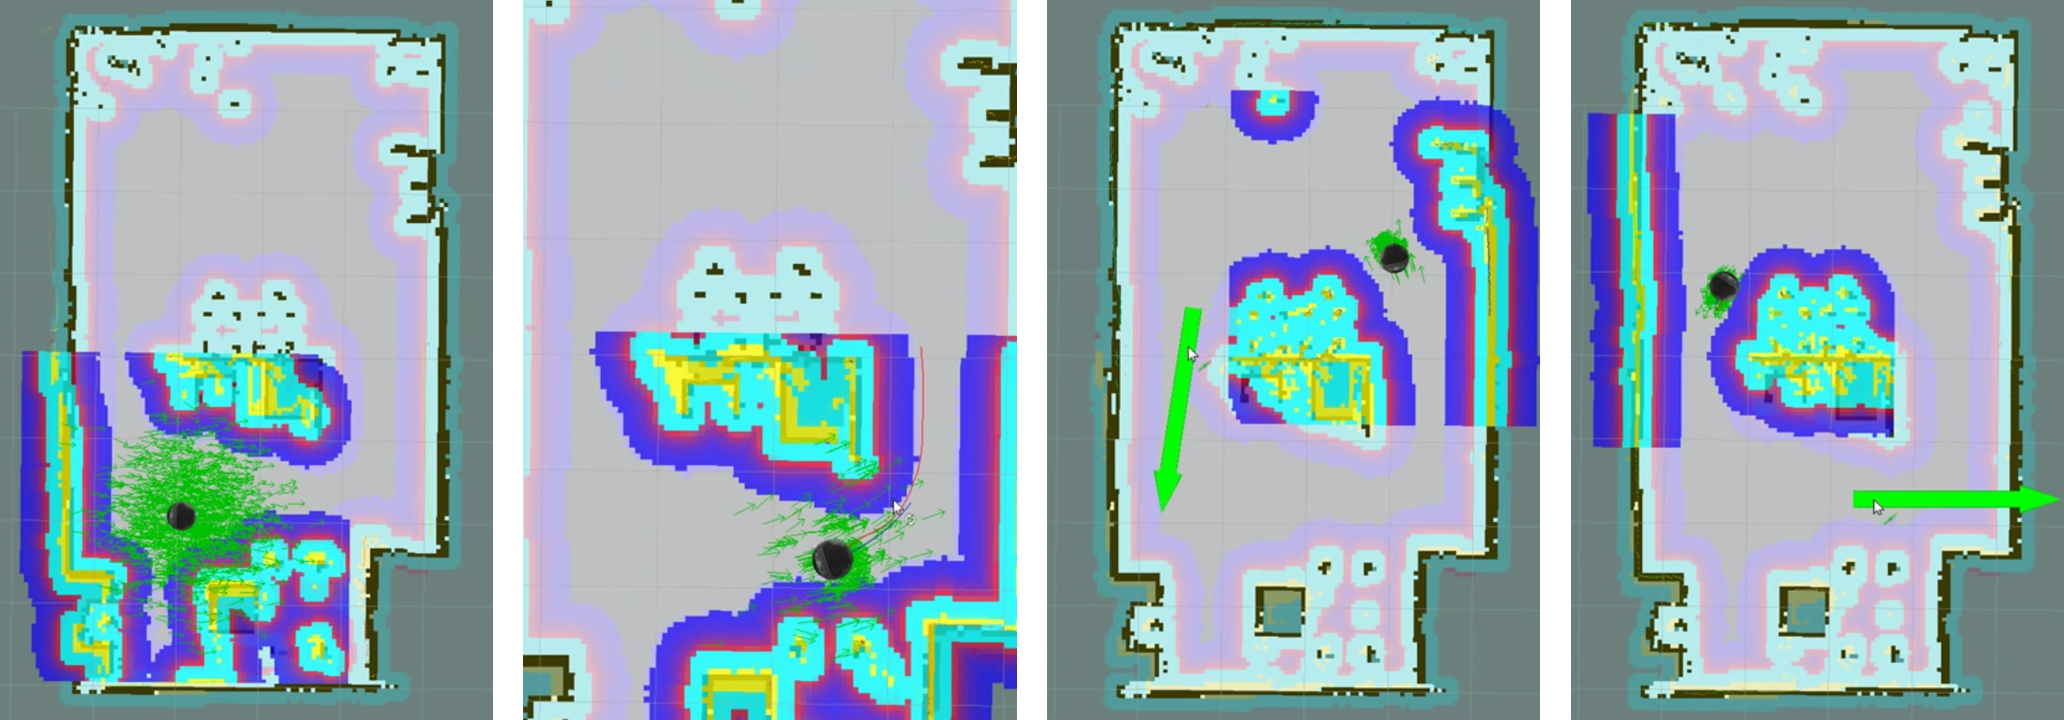
\includegraphics[width=\columnwidth]{pictures/chapter10/pic_10_14.png}
  \caption{目的地の設定 (左から3番目の図の大きな矢印)とロボットの移動の様子}
\end{figure}

初期位置と目的地の設定方法については、次のURLの動画を参考にしてほしい。 (URL: https://youtu.be/xCRsszVAP1E)
次節では、本節で実行したパッケージの詳細な説明と設定法について説明する。

%-------------------------------------------------------------------------------
\section{ROSを用いたナビゲーションの詳細}\index{ROSを用いたナビゲーションの詳細}

本節では、ナビゲーションで使用されるROSパッケージが、どのように作成、設定されているかについて解説する。取り上げるパッケージは、kobukiメタパッケージと、LRFのドライバであるurg\_nodeノード、座標変換のためのkobuki\_tfノード、Kobuki 3次元モデル (kobuki\_description)、環境地図を読み出すmap\_serverノード、AMCLノード、move\_baseノードになどである。
本節では、KobukiとLRFを用いた場合について説明するが、これを応用すれば、特定のロボットプラットフォームとセンサに限定されず、自作したロボットでもナビゲーションを使用できる。

%-------------------------------------------------------------------------------
\subsection{ナビゲーション  の手順}

ナビゲーションは、前述のように、環境地図が与えられた環境で、ロボットを現在地から指定された目的地まで移動させる方法である。したがって、ナビゲーションの実行には環境地図の存在が前提となる。環境地図の作成には、すでに説明したSLAMを用いることもできる。
環境地図が与えられた後、ナビゲーションは通常、以下の手順により行われる。

\setcounter{num}{0}

\stepcounter{num}\circled{\thenum} センシングと障害物検出

エンコーダや慣性センサ (IMU)から位置推定のための計測値を読み込む。また、距離センサで障害物 (壁、物体、家具など)を検出し、検出された障害物までの距離を計測する。

\stepcounter{num}\circled{\thenum} 位置推定

\circled{1} で得られたセンサ情報から、環境地図上でのロボットの現在位置を推定する。位置推定方法は多数あるが、本節ではMonte Carlo Localization (MCL)の一種であるパーティクルフィルタを用いたAMCL を利用する。

\stepcounter{num}\circled{\thenum} 経路計画

現在の位置から環境地図上で指定された目標の位置まで移動経路を計画する。ロボットの移動経路を作成する際には、環境地図全体の大域的な経路計画 (global path plannig)と、ロボットを中心とした局所的な経路計画 (local path plannig)に分けて考えるのが一般的である。本節では、障害物回避アルゴリズムであるDynamic Window Approach (DWA)注6を用いた、move\_baseとnav\_coreなどの経路計画パッケージを利用する。

\stepcounter{num}\circled{\thenum} 移動/障害物回避

運動計画で作成された移動経路をロボットに送り、ロボットはその経路に沿って目的地まで移動する。移動中に突然現れた障害物、移動物体などは、DWAアルゴリズムにより回避し、移動を継続する。

%-------------------------------------------------------------------------------
\subsection{ナビゲーションに必要な情報}

図10-15は、ROSのナビゲーションパッケージの実行に必要なノードとトピックの関係図である。ナビゲーションに必要な情報 (トピック)を中心に説明する。

\begin{figure}[htp]
  \centering
  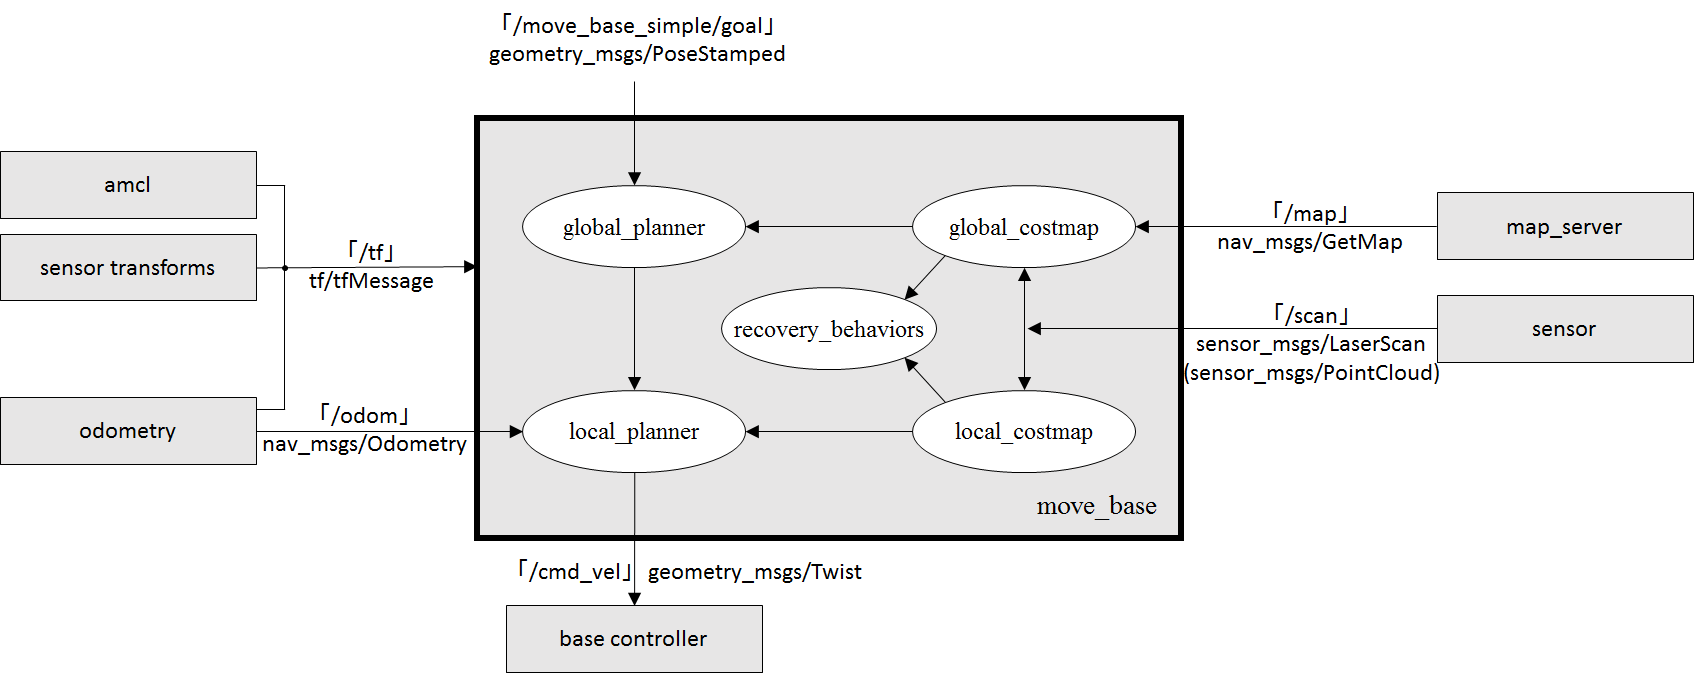
\includegraphics[width=\columnwidth]{pictures/chapter10/pic_10_15.png}
  \caption{ナビゲーションに必要なノードとトピックの関係図}
\end{figure}

\setcounter{num}{0}

\stepcounter{num}\circled{\thenum} オドメトリ (「/odom」、nav\_msgs/Odometry)

ロボットのオドメトリ情報は、センサ情報の変換の他、局所経路計画や障害物回避などに使用される。

\stepcounter{num}\circled{\thenum} 座標変換 (「/tf」、tf/tfMessage)

オドメトリ情報の基準点(odom)やロボット本体の基準点(base\_link)  、センサの取り付け位置(base\_scan)などの関係は、座標変換を表すtf情報で表現される。例えばセンサの取り付け位置は、odom → base\_linkfootprint → base\_link → base\_scanの変換を経て、tfトピック  として配信される。move\_baseノードでは、この情報を受けて、移動経路を計画することになる。

\stepcounter{num}\circled{\thenum} 距離センサ (「/scan」、sensor\_msgs/LaserScan or sensor\_msgs/PointCloud)

LRFやKinect、Xtionなどのセンサで測定された距離値を表す。この距離情報は、ロボットの位置推定法であるAMCLを利用して、ロボットの現在位置の推定やロボットの移動計画に使用される。本節では、このセンサの値を「scan」というトピック名で配信する。

\stepcounter{num}\circled{\thenum} 環境地図 (「/map」、nav\_msgs/GetMap)

map\_serverパッケージを利用して、10.2節  で作成した占有格子地図である「map.pgm」と「map.yaml」を配信する。

\stepcounter{num}\circled{\thenum} 目標座標 ( 「/move\_base\_simple/goal」、geometry\_msgs/PoseStamped)

目標座標は、ユーザーが直接指定する。本節では、ROSの可視化ツールであるRVizで目標座標を指定する。目標座標は、2次元座標 (x、y)と姿勢θで構成されている。

\stepcounter{num}\circled{\thenum} 速度コマンド (「/cmd\_vel」、geometry\_msgs/Twist)

計画された移動軌跡に基づき、速度コマンドを配信することで、ロボットは目的地まで移動する。本節では、この速度コマンドを「/mobile\_base/commands/velo\\city」というトピック名で配信する。

%-------------------------------------------------------------------------------
\subsection{kobuki\_navigationの実行}

10.5節で説明したとおり、次のkobuki\_nodeとkobuki\_navigationを実行し、ナビゲーションを実行しよう。

\begin{lstlisting}[language=ROS]
$ roslaunch kobuki_node minimal.launch --screen
$ roslaunch kobuki_navigation kobuki_navigation.launch --screen
\end{lstlisting}

ここで、rqt\_graphを実行すると、図10-16のようにROS環境で実行しているノードとトピックの情報が確認できる。ナビゲーションに必要な情報は、それぞれ/odom、/tf、/scan、/map、/mobile\_base/commands/velocityというトピック名で配信/購読されており、/move\_base\_simple/goalはRVizで目標座標を指定した後に配信される。

\begin{figure}[htp]
  \centering
  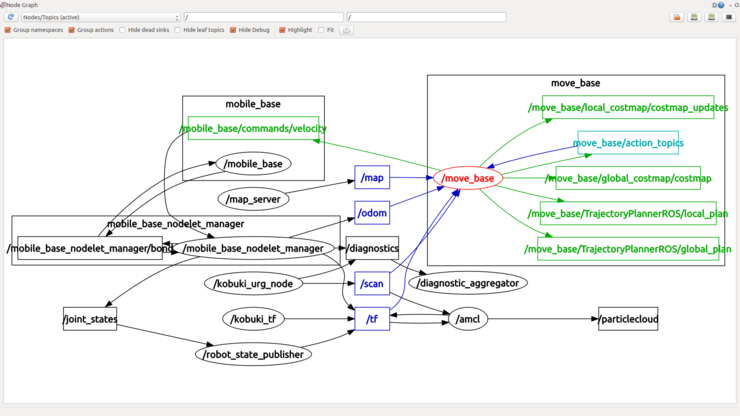
\includegraphics[width=15cm]{pictures/chapter10/pic_10_16.png}
  \caption{kobuki\_navigationの各ノードとトピックの状態}
\end{figure}

%-------------------------------------------------------------------------------
\subsection{kobuki\_navigationパッケージの作成}

本稿では、新たにkobuki\_navigationパッケージを作成する。まず、既存のkobuki\_na\\vigationパッケージを削除する

\begin{lstlisting}[language=ROS]
$ roscd kobuki_navigation
$ rm -r ./../kobuki_navigation
\end{lstlisting}

次に、新たにkobuki\_navigationというナビゲーションパッケージを作成しよう。

\begin{lstlisting}[language=ROS]
$ cd ~/catkin_ws/src/
$ catkin_create_pkg kobuki_navigation amcl move_base kobuki_node kobuki_tf urg_node map_server
\end{lstlisting}

コマンドの最後に続くオプションで「amcl move\_base kobuki\_node kobuki\_tf urg\_node map\_server」を指定しているが、これは「kobuki\_navigation」パッケージが依存しているパッケージを表す。
このパッケージを作成したディレクトリに、launchファイルを保存するlaunchフォルダ、作成されたマップを保存するmapsフォルダ、各種パラメータ情報を保存するparamフォルダ、RVizの設定情報ファイルを保存するrvizフォルダをそれぞれ作成する。  本パッケージは、既存のパッケージの設定だけで構成されているため、実質的にビルドすべきソースファイルはない。したがってsrcフォルダは省略する。

\begin{lstlisting}[language=ROS]
$ mkdir ./kobuki_navigation/launch ./kobuki_navigation/maps ./kobuki_navigation/param ./kobuki_navigation/rviz
\end{lstlisting}

ナビゲーションの実行には、ナビゲーションノードに関連するパッケージを起動するlaunchファイル、xmlファイル、各種パラメータの設定をするyamlファイル、環境地図関連ファイル、rviz設定ファイルが必要である。これらの構成ファイルの名前と役割 は、次の通りである。以下のファイルはhttps://github.com/irvs/r\\osbook\_kobukiで公開している。必要に応じて参照してほしい。

■ /launch/kobuki\_navigation.launch\\
kobuki\_navigation.launchファイルを実行するだけで、全てのナビゲーション関連パッケージが起動される。\\
■ /launch/amcl.launch.xml\\
amcl.launch.xmlファイルは、AMCL の各種パラメータの設定値を記述したファイルで、kobuki\_navigationl.launchと同時に使用される。\\
■ /param/move\_base\_params.yaml\\
運動計画を統括するmove\_baseのパラメータ設定ファイルである。\\
■ /param/costmap\_common\_params.yaml\\
■ /param/global\_costmap\_params.yaml\\
■ /param/local\_costmap\_params.yaml\\
占有格子地図の設定パラメータを記載したファイルであり、大域経路計画に関するglobal\_costmap\_params.yaml、局所経路計画に関するlocal\_costmap\_params.yamlファイル、両者に共通のcostmap\_common\_params.yamlファイルからなる。本節で用いる占有格子地図では、costmap注7という手法を用いて、ロボットの位置情報とセンサから得られた周辺情報から、各ピクセルを障害物、移動不可領域、移動可能領域に分類する。この分類に必要なcostmapの設定パラメータが記載されている。\\
■ /param/dwa\_local\_planner\_params.yaml\\
dwa\_local\_plannerは計画された移動速度コマンドをロボットに送るパッケージで、このパッケージの実行に必要なパラメータ  を設定するファイルである。\\
■ /maps/map.pgm\\
■ /maps/map.yaml\\
以前10.2節で  作成した占有格子地図である「map.pgm」と、その環境地図情報である「map.yaml」をmapsフォルダに保存して使用する。\\
■ /rviz/kobuki\_nav.rviz\\
RVizの設定情報を含むファイルである。RVizのプラグインとして、Grid、RobotModel、TF、LaserScan、Bumper Hit、Map、Global Map、Local Map、AMCL Particlesを呼び出す。

%-------------------------------------------------------------------------------
\subsection{kobuki\_navigationの設定}

kobuki\_navigation.launchファイルの設定について説明する。まずはファイル全体を示す。

\textbf{ファイル名: /launch/kobuki\_navigation.launch}
\begin{lstlisting}[language=XML]
<launch>
  <!-- kobuki model -->
  <arg name="urdf_file" default="$(find xacro)/xacro.py
'$(find kobuki_description)/urdf/kobuki_standalone.urdf.xacro'" />
  <param name="robot_description" command="$(arg urdf_file)" />
  <node pkg="robot_state_publisher" type="robot_state_publisher" name="robot_state_publisher" output="screen">
    <param name="publish_frequency" type="double" value="5.0" />
  </node>

  <!-- sensor -->
  <node pkg="urg_node" type="urg_node" name="kobuki_urg_node" output="screen">
    <param name="frame_id" value="base_scan" />
  </node>

  <!-- tf -->
  <node pkg="kobuki_tf" type="kobuki_tf" name="kobuki_tf" output="screen">
  </node>

  <!-- Map server -->
  <arg name="map_file" default="$(find kobuki_navigation)/maps/map.yaml"/>
  <node name="map_server" pkg="map_server" type="map_server" args="$(arg map_file)">
  </node>

  <!-- AMCL -->
  <include file="$(find kobuki_navigation)/launch/amcl.launch.xml"/>

  <!-- move_base -->
  <arg name="cmd_vel_topic" default="/mobile_base/commands/velocity" />
  <arg name="odom_topic" default="odom" />
  <node pkg="move_base" type="move_base" respawn="false" name="move_base" output="screen">
    <rosparam file="$(find kobuki_navigation)/param/costmap_common_params.yaml" command="load" ns="global_costmap" />
    <rosparam file="$(find kobuki_navigation)/param/costmap_common_params.yaml" command="load" ns="local_costmap" />
    <rosparam file="$(find kobuki_navigation)/param/local_costmap_params.yaml" command="load" />
    <rosparam file="$(find kobuki_navigation)/param/global_costmap_params.yaml" command="load" />
    <rosparam file="$(find kobuki_navigation)/param/dwa_local_planner_params.yaml" command="load" />
    <rosparam file="$(find kobuki_navigation)/param/move_base_params.yaml" command="load" />
    <remap from="cmd_vel" to="$(arg cmd_vel_topic)"/>
    <remap from="odom" to="$(arg odom_topic)"/>
  </node>
</launch>
\end{lstlisting}

\subsubsection{Kobukiの3次元モデル (kobuki model)}

最初の項目は、kobuki\_descriptionパッケージでkobuki\_standalone.urdfの3Dモデルを呼び出し、robot\_state\_publisherを介して車輪角度情報などのロボットの状態をtfトピックで配信するものである。この設定により、RVizの画面にKobukiの3次元モデルを表示できる。

\begin{lstlisting}[language=XML]
<arg name="urdf_file" default="$(find xacro)/xacro.py
'$(find kobuki_description)/urdf/kobuki_standalone.urdf.xacro'" />
<param name="robot_description" command="$(arg urdf_file)" />
<node pkg="robot_state_publisher" type="robot_state_publisher" name="robot_state_publisher" output="screen">
  <param name="publish_frequency" type="double" value="5.0" />
</node>
\end{lstlisting}

\subsubsection{センサ (sensor)}

urg\_nodeノードを実行し、Kobukiに装着されたLRFを起動する。paramオプションにより「frame\_id」パラメータを「base\_scan」に変換して実行する。

\begin{lstlisting}[language=XML]
<node pkg="urg_node" type="urg_node" name="kobuki_urg_node" output="screen">
  <param name="frame_id" value="base_scan" />
</node>
\end{lstlisting}

\subsubsection{相対座標変換 (tf)}

kobuki\_tfノードは、オドメトリ情報 (odom)からセンサ取り付け位置 (base\_scan)までの座標変換 (odom → base\_footprint → base\_link → base\_scan)情報をtfトピック  で配信する。

\begin{lstlisting}[language=XML]
<node pkg="kobuki_tf" type="kobuki_tf" name="kobuki_tf" output="screen"> </node>
\end{lstlisting}

\subsubsection{環境地図サーバ (Map server)}

map\_serverノードを実行し、kobuki\_navigation/mapsフォルダに保存された環境地図情報 (map.yaml)を読み込み、環境地図を配信する。

\begin{lstlisting}[language=XML]
<arg name="map_file" default="$(find kobuki_navigation)/maps/map.yaml"/>
<node name="map_server" pkg="map_server" type="map_server" args="$(arg map_file)">
</node>
\end{lstlisting}

\subsubsection{AMCL}

AMCL関連のamclノードを実行する。

\begin{lstlisting}[language=XML]
<include file="$(find kobuki_navigation)/launch/amcl.launch.xml"/>
\end{lstlisting}

\subsubsection{move\_base}

動作計画を行うmove\_baseノードを実行する。この際、costmap関連パラメータやdwa\_local\_plannerのパラメータ、運動計画を行うmove\_baseのパラメータを設定する。  この設定については、次項で詳しく説明する。

\begin{lstlisting}[language=XML]
<arg name="cmd_vel_topic" default="/mobile_base/commands/velocity" />
<arg name="odom_topic" default="odom" />

<node pkg="move_base" type="move_base" respawn="false" name="move_base" output="screen">
  <rosparam file="$(find kobuki_navigation)/param/costmap_common_params.yaml" command="load" ns="global_costmap" />
  <rosparam file="$(find kobuki_navigation)/param/costmap_common_params.yaml" command="load" ns="local_costmap" />
  <rosparam file="$(find kobuki_navigation)/param/local_costmap_params.yaml" command="load" />
  <rosparam file="$(find kobuki_navigation)/param/global_costmap_params.yaml" command="load" />
  <rosparam file="$(find kobuki_navigation)/param/dwa_local_planner_params.yaml" command="load" />
  <rosparam file="$(find kobuki_navigation)/param/move_base_params.yaml" command="load" />
  <remap from="cmd_vel" to="$(arg cmd_vel_topic)"/>
  <remap from="odom" to="$(arg odom_topic)"/>
</node>
\end{lstlisting}

%-------------------------------------------------------------------------------
\subsection{kobuki\_navigation関連の詳細パラメータ設定}

この項では、kobuki\_navigationに関連した詳細なパラメータを設定する方法を説明する。

\subsubsection{AMCL}

amcl.launch.xmlファイルはAMCLのパラメータ設定値が入ったファイルで、前述のkobuki\_navigation.launchと同時に使用される。AMCLの説明は、10.7節  で行う。

\textbf{ファイル名: /launch/amcl.launch.xml}
\begin{lstlisting}[language=XML]
<launch>
<!-- %*trueの場合は、ACMLはマップのトピックを受信し、falseであればstatic\_mapのサービス*)
%*コールを使用する。 *) -->
<arg name = "use_map_topic" default = "false" />
<!-- %*距離センサからの距離値のトピック名 *) -->
<arg name = "scan_topic" default = "scan" />
<!-- %*初期位置推定で使われるガウス分布のx座標値 *) -->
<arg name = "initial_pose_x" default = "0.0" />
<!-- %*初期位置推定で使われるガウス分布のy座標値 *) -->
<arg name = "initial_pose_y" default = "0.0" />
<!-- %*初期位置推定で使われるガウス分布のyaw値 *) -->
<arg name = "initial_pose_a" default = "0.0" />

<!-- %*下のパラメータ設定を参考し、amclノードを実行する。 *) -->
<node pkg = "amcl" type = "amcl" name = "amcl">

<!-- %*フィルタ関連パラメータ *) -->
<!-- %*最小のパーティクル数 *) -->
<param name = "min_particles" value = "500" />
<!-- %*最大のパーティクル数 (多いほど良い、PCのパフォーマンスに応じて設定) *) -->
<param name = "max_particles" value = "2000" />
<!-- %*実際の分布と推定された分布の間の最大エラー *) -->
<param name = "kld_err" value = "0.05" />
<!-- %*フィルタの更新に必要な並進運動 (メートル単位) *) -->
<param name = "update_min_d" value = "0.25" />
<!-- %*フィルタの更新に必要な回転運動 (ラジアン単位) *) -->
<param name = "update_min_a" value = "0.2" />
<!-- %*再サンプリング間隔 *) -->
<param name = "resample_interval" value = "1" />
<!-- %*変換許容時間 (秒単位) *) -->
<param name = "transform_tolerance" value = "1.0" />
<!-- %*指数の減少率 (slow average weight filter) *) -->
<param name = "recovery_alpha_slow" value = "0.0" />
<!-- %*指数の減少率 (fast average weight filter) *) -->
<param name = "recovery_alpha_fast" value = "0.0" />
<!-- %*上記initial\_pose\_xの説明を参照 *) -->
<param name = "initial_pose_x" value = "$ (arg initial_pose_x)" />
<!-- %*上記initial\_pose\_yの説明を参照 *) -->
<param name = "initial_pose_y" value = "$ (arg initial_pose_y)" />
<!-- %*上記innitial\_pose\_aの説明を参照 *) -->
<param name = "initial_pose_a" value = "$ (arg initial_pose_a)" />

<!-- %*スキャンや移動経路の情報  を視覚的に表示する周期 (10Hz = 0.1秒) *) -->
<param name = "gui_publish_rate" value = "10.0" />
<!-- %*上記use\_map\_topicの説明と同じ *) -->
<param name = "use_map_topic" value = "$ (arg use_map_topic)" />

<!-- %*距離センサパラメータ *) -->
<!-- %*センサトピック名の変更 *) -->
<remap from = "scan" to = "$ (arg scan_topic)" />
<!-- %*レーザーの最大距離 (センサに合わせて設定する、メートル単位) *) -->
<param name = "laser_max_range" value = "10.0" />
<!-- %*フィルタが更新されるときに使用されている最大のレーザービームの数 *) -->
<param name = "laser_max_beams" value = "60" />
<!-- %*センサモデルのz\_hit混合重み (micture weight) *) -->
<param name = "laser_z_hit" value = "0.5" />
<!-- %*センサのz\_short混合重み (micture weight) *) -->
<param name = "laser_z_short" value = "0.05" />
<!-- %*センサのz\_max混合重み (micture weight) *) -->
<param name = "laser_z_max" value = "0.05" />
<!-- %*センサのz\_rand混合重み (micture weight) *) -->
<param name = "laser_z_rand" value = "0.5" />
<!-- %*センサのz\_hitを使用したガウスモデルの標準偏差 *) -->
<param name = "laser_sigma_hit" value = "0.2" />
<!-- %*センサのz\_shortの指数関数パラメータ *) -->
<param name = "laser_lambda_short" value = "0.1" />
<!-- %*likelihood\_field方式センサのための障害物との最大距離 *) -->
<param name = "laser_likelihood_max_dist" value = "2.0" />
<!-- %*センサタイプ (likelihood\_fieldとbeam選択) *) -->
<param name = "laser_model_type" value = "likelihood_field" />

<!-- %*オドメトリ関連パラメータ *) -->
<!-- %*ロボット移動方式の "diff"と "omni"が選択可能である。 *) -->
<param name = "odom_model_type" value = "diff" />
<!-- %*回転運動のとき、予想されるオドメトリの回転運動量推定ノイズ *) -->
<param name = "odom_alpha1" value = "0.2" />
<!-- %*並進運動のとき、予想されるオドメトリの回転運動量推定ノイズ *) -->
<param name = "odom_alpha2" value = "0.2" />
<!-- %*並進運動のとき、予想されるオドメトリの並進運動量推定ノイズ *) -->
<param name = "odom_alpha3" value = "0.2" />
<!-- %*回転運動のとき、予想されるオドメトリの並進運動量推定ノイズ *) -->
<param name = "odom_alpha4" value = "0.2" />
<!-- %*オドメトリフレームID *) -->
<param name = "odom_frame_id" value = "odom" />
<!-- %*ロボットベースフレームID *) -->
<param name = "base_frame_id" value = "base_footprint" />

</ node>
</ launch>
\end{lstlisting}

\subsubsection{move\_base}

動作計画を統括するmove\_baseのパラメータ設定ファイルである。

\textbf{ファイル名: /param/move\_base\_params.yaml}
\begin{lstlisting}[language=YAML]
# %*move\_baseが無効な場合costmapノードを停止させるかの選択*)
shutdown_costmaps: false
# %*ロボットベースに速度コマンドを与えるコントロール繰り返しの周期 (Hz単位)*)
controller_frequency: 5.0
# %*space-clearing動作が実行される前に、コントローラが制御情報を受信待機する最大時間*)
controller_patience: 3.0
# %*全域計画の繰り返し周期 (Hz単位)*)
planner_frequency: 1.0
# %*space-clearing動作前に、使用可能な計画を見つけるために待機する最大時間*)
planner_patience: 5.0
# %*回復行動    (軌道計画に失敗した時の行動)を実行する前に、ロボットが行ったり来たりするこ*)
%*とを可能にする時間*)
oscillation_timeout: 10.0
# %*この距離を移動した場合、oscillation\_timeoutは初期化される。*)
oscillation_distance: 0.2
\end{lstlisting}

\subsubsection{costmap}

共通のcostmap\_common\_params.yamlファイル、大域経路計画に必要なglobal\_cost\\map\_params.yaml、局所経路計画に必要なlocal\_costmap\_params.yamlファイルの設定について説明する。

\textbf{ファイル名: /param/costmap\_common\_params.yaml}
\begin{lstlisting}[language=YAML]
# %*センサの値のうち、この距離値より近いとき、障害物として処理する。以下メートル単位*)
obstacle_range: 2.5
# %*センサの値のうち、この距離値以上のデータは無視される。*)
raytrace_range: 3.0
# %*ロボット半径*)
robot_radius: 0.18
# %*インフレーション領域    (ロボットの近傍領域)を表す円の半径で、障害物へ接近させないよう*)
%*にするパラメータ*)
inflation_radius: 0.50
# %*使用するcostmapをvoxel (voxel-grid)とcostmap (costmap\_2d)の中から選択する。*)
map_type: voxel
# %*初期高さの値*)
origin_z: 0.0
# %*各ボクセル   (3次元空間を構成する小6面体)の高さ*)
z_resolution: 0.2
# %*ボクセルの種類数を指定、以下のように2を設定すると、0と1が使える。ボクセル0はバンパ*)
  %*ーが使用され、ボクセル1はレーザースキャナが使用される。*)
z_voxels: 2
# %*ボクセルマップを配信するかどうかを決定*)
publish_voxel_map: false
# %*障害物の最大高さ (ロボットアームを装着した場合を考慮すること)*)
max_obstacle_height: 0.60
# %*使用するセンサの指定*)
observation_sources: scan bump
# %*レーザスキャンのデータのタイプ、トピック名、costmapへの反映、最小・最大の障害物の*)
%*高さについてのパラメータ*)
scan: {data_type: LaserScan, topic: scan, marking: true, clearing: true, min_obstacle_height: 0.25, max_obstacle_height: 0.35}
# %*バンパーのデータのタイプ、トピック名、costmapへの反映、最小・最大の障害物の高さに*)
%*ついてのパラメータ*)
bump: {data_type: PointCloud2, topic: mobile_base/sensors/bumper_pointcloud, marking: true, clearing: false, min_obstacle_height: 0.0, max_obstacle_height: 0.15}
\end{lstlisting}

\textbf{ファイル名: /param/global\_costmap\_params.yaml}
\begin{lstlisting}[language=YAML]
global_costmap:
 global_frame: /map        #%*マップフレームの設定*)
 robot_base_frame: /base_footprint #%*ロボットベースフレームの設定*)
 update_frequency: 1.0     #%*更新周期 (Hz)*)
 publish_frequency: 0.5      #%*配信サイクル (秒)*)
 static_map: true        #%*指定したマップを使用するかの設定*)
 transform_tolerance: 0.5      #%*変換許容距離 (メートル)*)
\end{lstlisting}

\textbf{ファイル名: /param/local\_costmap\_params.yaml}
\begin{lstlisting}[language=YAML]
local_costmap:
 global_frame: /map        #%*マップフレームの設定*)
 robot_base_frame: /base_footprint #%*ロボットベースフレームの設定*)
 update_frequency: 5.0      #%*更新周期 (Hz)*)
 publish_frequency: 2.0       #%*配信サイクル (Hz)*)
 static_map: false        #%*指定したマップを使用するかの設定*)
 rolling_window: true       #%*局所環境地図ウィンドウの使用設定*)
 width: 4.0           #%*局所環境地図ウィンドウの横 (メートル)*)
 height: 4.0          #%*局所環境地図ウィンドウの縦 (メートル)*)
 resolution: 0.05         #%*局所環境地図ウィンドウの解像度 (メートル/セル)*)
 transform_tolerance: 0.5       #%*変換許容距離 (メートル)*)
\end{lstlisting}

\subsubsection{dwa\_local\_planner}

dwa\_local\_plannerは移動速度コマンドをロボットに送るパッケージで、dwa\_local\\\_planner\_params.yamlはパラメータを設定するファイルである。この詳細設定について説明する。

\textbf{ファイル名: /param/dwa\_local\_planner\_params.yaml}
\begin{lstlisting}[language=YAML]
DWAPlannerROS:

#%*ロボットパラメータ設定 (Kobuki)*)
max_vel_x: 0.5   #%*x軸の最大速度 (meter/sec)*)
min_vel_x: 0.0   #%*x軸の最小速度 (meter/sec)*)

max_vel_y: 0.0   #%*全方向ロボットの場合に設定*)
min_vel_y: 0.0   #%*全方向ロボットの場合に設定*)

max_trans_vel: 0.5   #%*最大並進速度 (meter/sec)*)
min_trans_vel: 0.1   #%*最小並進速度 (meter/sec)*)
trans_stopped_vel: 0.1 #%*停止並進速度 (meter/sec)*)

max_rot_vel: 5.0   #%*最大回転速度 (radian/sec)*)
min_rot_vel: 0.4   #%*最小回転速度 (radian/sec)*)
rot_stopped_vel: 0.4 #%*停止回転速度 (radian/sec)*)

acc_lim_x: 1.0   #%*x軸加速度制限 (meter/sec\^2)*)
acc_lim_y: 0.0   #%*y軸加速度制限 (meter/sec\^2)*)

#%*目標地点の許容誤差*)
yaw_goal_tolerance: 0.3  #%*yaw軸の角度許容誤差 (radian)*)
xy_goal_tolerance: 0.15  #%*x、y座標の距離許容誤差 (meter)*)

#%*フォワードシミュレーション (Forward Simulation)パラメータ*)
sim_time: 1.0      #%*フォワードシミュレーション軌跡時間*)
vx_samples: 6      #%*x軸速度空間で探索するサンプル数*)
vy_samples: 1      #%*y軸速度空間で探索するサンプル数*)
vtheta_samples: 20   #%*yaw軸   速度空間で探索するサンプル数*)

#%*軌跡スクロールパラメータ (軌跡評価)*)
path_distance_bias: 64.0 #%*コントローラのパス追従の重み*)
goal_distance_bias: 24.0 #%*目標地点と制御速度に近いかどうかの重み*)
occdist_scale: 0.5   #%*障害物回避のための重み*)
forward_point_distance: 0.325  #%*ロボットから追加スクロール点との距離 (meter)*)
stop_time_buffer: 0.2  #%*ロボット停止に必要な時間 (sec)*)
scaling_speed: 0.25    #%*スケーリング速度 (meter/sec)*)
max_scaling_factor: 0.2  #%*最大スケーリング係数*)

#%*不安定な挙動 (Oscillation)を防ぐためのパラメータ*)
oscillation_reset_dist: 0.05 #%*oscillationフラグがリセットされる前に、ロボットがどのように移動*)
%*するかの設定*)

#%*デバッグ*)
publish_traj_pc: true    #%*移動軌跡のデバッグ設定*)
publish_cost_grid_pc: true   #%*costmapデバッグ設定*)
global_frame_id: odom    #%*グローバルフレームIDの設定*)
\end{lstlisting}

\subsubsection{map}

以前に作成した占有格子地図をmapsフォルダに保存して使用する。特別な設定パラメータはない。

\begin{itemize}
\item /maps/map.pgm
\item /maps/map.yaml
\end{itemize}

\subsubsection{kobuki\_nav.rviz}

RVizの設定情報を含むファイルである。 RVizのプラグインで、Grid、RobotMode\\l、TF、LaserScan、Bumper Hit、Map、Global Map、Local Map、Amcl Particlesを呼び出す。RViz起動後に、図10-17のように「Add」ボタンを押して手動で追加することもできるが、より簡便に起動時に自動で  追加するための設定ファイルを下記アドレスからダウンロードできる。

\begin{lstlisting}[language=ROS]
$ wget https://raw.githubusercontent.com/irvs/rosbook_kobuki/master/kobuki_navigation/rviz/kobuki_nav.rviz
$ cp kobuki_nav.rviz `rospack find kobuki_slam`/rviz/
$ rosrun rviz rviz -d `rospack find kobuki_slam`/rviz/kobuki_nav.rviz
\end{lstlisting}

\begin{figure}[htp]
  \centering
  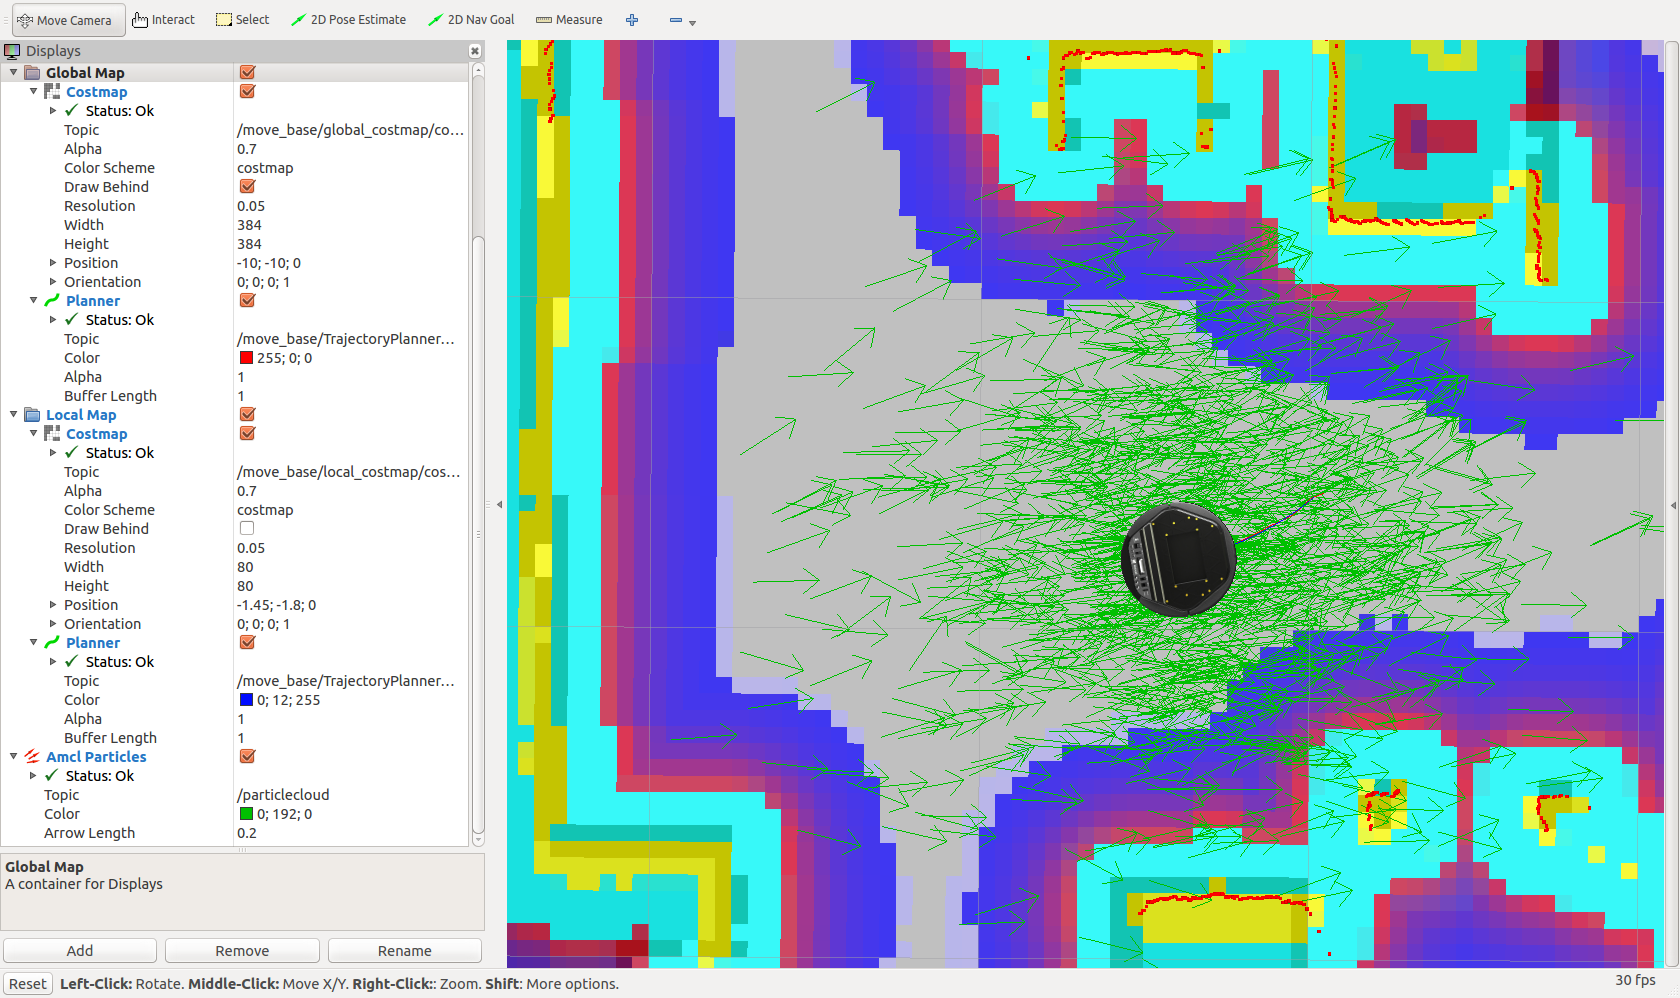
\includegraphics[width=12cm]{pictures/chapter10/pic_10_17.png}
  \caption{RVizでのナビゲーションの様子}
\end{figure}

以上で、ナビゲーションパッケージを使用するために必要な手順を説明した。次節では、costmap、AMCL、DWAについて説明する。

%-------------------------------------------------------------------------------
\section{ナビゲーションの要素技術}\index{ナビゲーションの要素技術}

%-------------------------------------------------------------------------------
\subsection{Costmap}

ナビゲーションでは、エンコーダや慣性センサ (IMU)などのオドメトリ情報、距離センサによる障害物との距離情報、および与えられた占有格子地図の3種類の情報から、障害物領域や障害物との衝突が予想される領域、移動可能な領域を計算し、costmapに格納する。costmapは、用いられるナビゲーションの種類に応じて、2種類に分けられる。一つは、占有格子地図の全領域を対象にした大域経路計画で用いられるglobal\_costmapである  。もう一つは、ロボット近傍の局所経路計画に用いられるlocal\_costmapで、環境に適合した詳細な移動計画  や障害物回避時に使用される。global\_costmap とlocal\_costmapは使用目的が異なるだけで、表現方式は共通である。
costmapは、各領域の状態を0〜255の数値で表現する。  図10-18に、それぞれの値に対応する領域の種類を示す。直観的には、10.6節で説明したcostmap設定パラメータを用いて、ロボットが移動可能な領域か、あるいは障害物に衝突する可能性の高い領域かを表す。一例を以下に示す。

\begin{itemize}
\item 000: ロボットが移動可能な自由空間 (free area)
\item 001〜127: 衝突する可能性が低い領域
\item 128〜252: 衝突する可能性が高い領域
\item 253〜254: 衝突領域
\item 255: ロボットが移動不可能な占有空間 (occupied area)
\end{itemize}

\begin{figure}[htp]
  \centering
  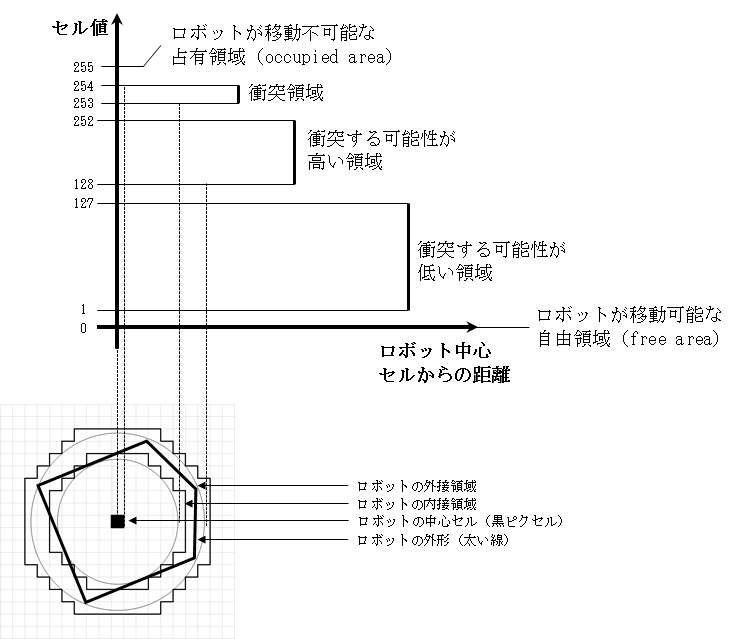
\includegraphics[width=12cm]{pictures/chapter10/pic_10_18.png}
  \caption{障害物との距離とcostmap値の関係}
\end{figure}

costmapを視覚的に表現すると、例えば図10-19のようになる。左図は地図をグレースケールで表示したもので、右図はカラーで表示したものである (「http://goo.gl/tlMnzv」を参照)。左図は中央にロボットがあり、地図の色が濃い領域ほど  衝突の可能性が高い。ロボット周囲の緑色  の枠がロボットのモデルであり、この緑の円が壁にぶつかると、ロボットは衝突する。赤は距離センサで得られた障害物である。
右図では、黄色の領域は障害物である。水色の領域はロボットの重心位置がこの中に入ると障害物と衝突することを示す。青の領域は衝突の可能性が低い  領域であり、紫は水色と青の  境界線である。

\begin{figure}[htp]
  \centering
  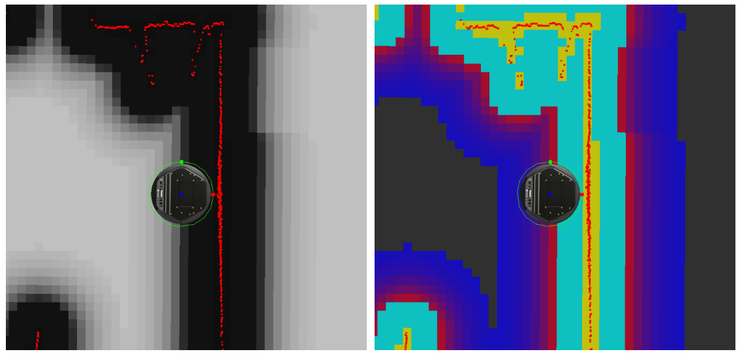
\includegraphics[width=10cm]{pictures/chapter10/pic_10_19.png}
  \caption{costmap表現 (「http://goo.gl/tlMnzv」を参照)}
\end{figure}

%-------------------------------------------------------------------------------
\subsection{MCL}

10.4節のSLAMの要素技術のパーティクルフィルタの項で述べたように、モンテカルロ位置推定アルゴリズムは、移動ロボットの位置推定で広く使用される。AMCLはモンテカルロ位置推定アルゴリズムの一種で、最適な数のサンプルを用いることで実行時間を減らし、リアルタイム性を高めたものである。ここでは、基本となるモンテカルロ位置推定について説明する。
モンテカルロ位置推定 (以下MCL)の目的は、与えられた環境の中でロボットがどこにいるか、すなわち環境地図上のロボットの座標 $(x, y)$と姿勢θ $\theta$を求めることである。そのためにMCLでは、ロボットの位置 を確率分布で表す。
 時刻tでのロボットの位置と姿勢 $(x, y, \theta)$を$x_t$ とし、時刻$t$までに  距離センサから得られた距離情報を「 $z_{0...t} = \{z_0, z_1, ..., z_t\}$」、時刻$t$までに  エンコーダから得られたロボットの移動情報を「$u_{0...t} = \{u_0, u_1, ..., u_t\}$」とする。このとき、次のように現在の推定位置でのbelief (ベイズの定理における事後確率)  を計算する。

 \begin{equation}
   bel(x_t) = P(x_t|z_{0\cdots t},u_{0\cdots t})
 \end{equation}

この計算は、センサモデルとロボットの移動モデルを分離して、ベイズフィルタの予測と更新により行う。まず予測処理では、ロボットの移動モデル「 $p( x_t | x_{(t-1)}, u_{(t-1)} )$」と、前時刻の位置の確率「$bel(x_{(t-1)})$」、エンコーダから得られた移動情報「$u_{(t-1)}$」を利用して、観測結果が得られる前の現時刻の位置の確率「$bel'(x_t)$」を計算する。

\begin{equation}
  bel'(x_t) = \int p(x_t | x_{t-1},u_{t-1})bel(x_{t-1})dx_{t-1}
\end{equation}

更新処理では、センサモデル「 $p( z_t | x_t )$」、観測結果が得られる前の位置の確率「$bel'(x_t)$bel'(xt)」、正規化定数「$(\eta_t)$」を用いて、ベイズの定理により観測結果ztが得られた時の位置の確率「$bel(x_t)$」を求める。

\begin{equation}
  bel(x_t) = \eta_t p(z_t|x_t)bel'(x_t)
\end{equation}

この現在の推定位置の確率「$bel(x_t)$」を利用して、パーティクルフィルタで位置を推定する。パーティクルフィルタについては、10.4.2項のパーティクルフィルタを参照してほしい。まず、多数のサンプル「$x_{t-1}^{\prime(i)}$」からなるサンプルセットXt-1を用意する。前時刻の位置の確率「$bel(x_{t-1})$」、ロボットの移動モデル「$p( x_t | x_{(t-1)}, u_{(t-1)}$」を用いて、新しいサンプルセット「${X’}_t$」を得る。次に、このサンプルセット「 $X{’}_t$」のサンプルiである「${x’}_t^{(i)}$」と、距離センサから得られた距離情報「$z_t$」、正規化定数「$\eta$」から、サンプルiの重み「$\omega_t^{(i)}$」を求める。

\begin{equation}
  \omega_t^{(i)} = \eta p(z_t|x_t^{\prime(i)})
\end{equation}

最後に、再サンプリング過程では、サンプル「${x’}_t^{(i)}$」と重み「$w_t^{(i)}$」を利用して、新しいサンプルセット$X_t$を作成する。

\begin{equation}
  X_t = \{x_t^{(j)} | j=1 \cdots N\} \sim \{x_t^{\prime(i)},\omega_t^{(i)}\}
\end{equation}

このように予測と更新を繰り返しながらパーティクルを収束させ、ロボットの推定位置を得る。一例を図10-20に示す。$t_1, t_2, t_3, t_4$と時刻が進むにつれて、パーティクルが収束していく様子がわかる。

\begin{figure}[htp]
  \centering
  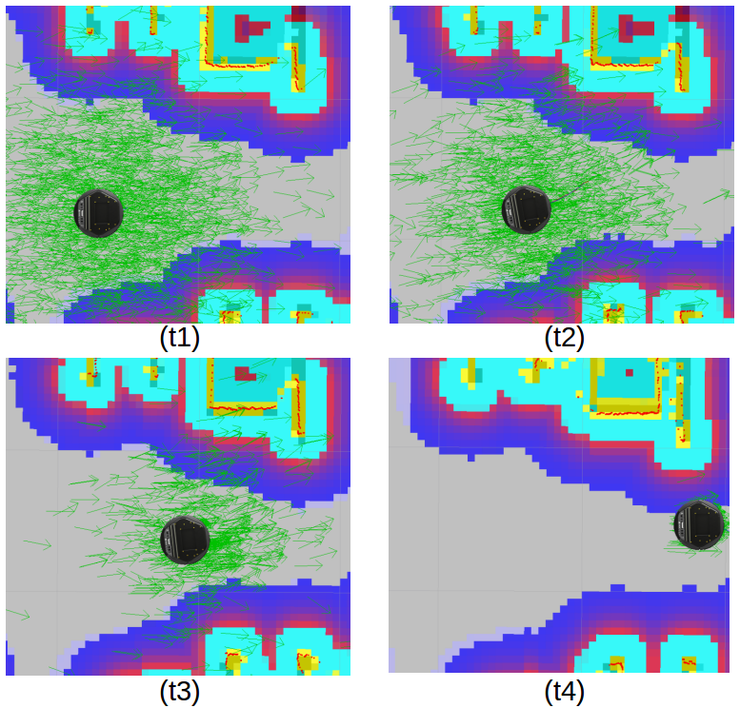
\includegraphics[width=12cm]{pictures/chapter10/pic_10_20.png}
  \caption{AMCLを用いたロボットの位置推定}
\end{figure}


%-------------------------------------------------------------------------------
\subsection{Dynamic Window Approach (DWA)}

Dynamic Windows Approach (DWA)は、ロボットの速度探索空間 (velocity search space)内で、衝突する可能性のある障害物を回避しながら目標位置へ到達する経路  を選択する方法である。
 図10-21のように、並進速度vと回転速度ωを軸とする速度探索空間 でロボットの経路を考える。この速度空間では、ロボットのハードウェアの制限上、現在の速度から到達可能な速度領域が存在し、この領域をダイナミックウィンドウ (Dynamic Window)と呼ぶ。他の記号は以下の意味を持つ。

\begin{itemize}
\item $V_s$: 最大速度領域
\item $V_a$: 許容速度領域
\item $V_c$: 現在の速度
\item $V_r$: ダイナミックウィンドウ内の速度領域
\item $a_max$: 最大加減速度
\end{itemize}

\begin{itemize}
\item  $G(v,\omega) = \sigma(\alpha heading(v,\omega) + \beta dist(v,\omega) + \gamma velocity(v,\omega))$: 目的関数
\item $heading(v,\omega)$: 180度-ロボットの方位とゴール方向の差
\item $dist(v,\omega)$: 障害物までの距離
\item $velocity(v,\omega)$: 選択された速度
\item $\alpha, \beta, \gamma$: 各項の重み
\item $\sigma(x)$: スムージング関数
\end{itemize}

このダイナミックウィンドウ内で、ロボットの方向、障害物までの距離、速度からなる目的関数G(v,ω)が最大となる並進速度vと回転速度ωを求める。すなわち、図10-22のように、実現可能な様々な進速度v、回転速度ωをの選択肢から、目標値に到達するために目的関数が最大となる  速度を得る。

\begin{figure}[htp]
  \centering
  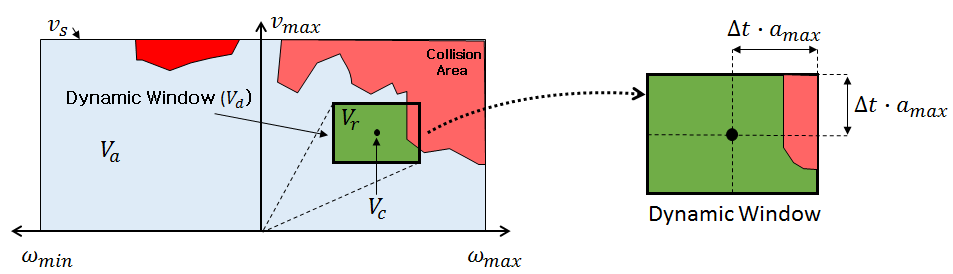
\includegraphics[width=12cm]{pictures/chapter10/pic_10_21.png}
  \caption{ロボットの速度探索空間 (velocity search space)とダイナミックウィンドウ}
\end{figure}

ここまで、SLAMとナビゲーションについて説明した。移動ロボットプラットフォームKobukiを中心に説明したが、他の移動ロボットプラットフォームや独自のロボットにも適用できる。

\begin{figure}[htp]
  \centering
  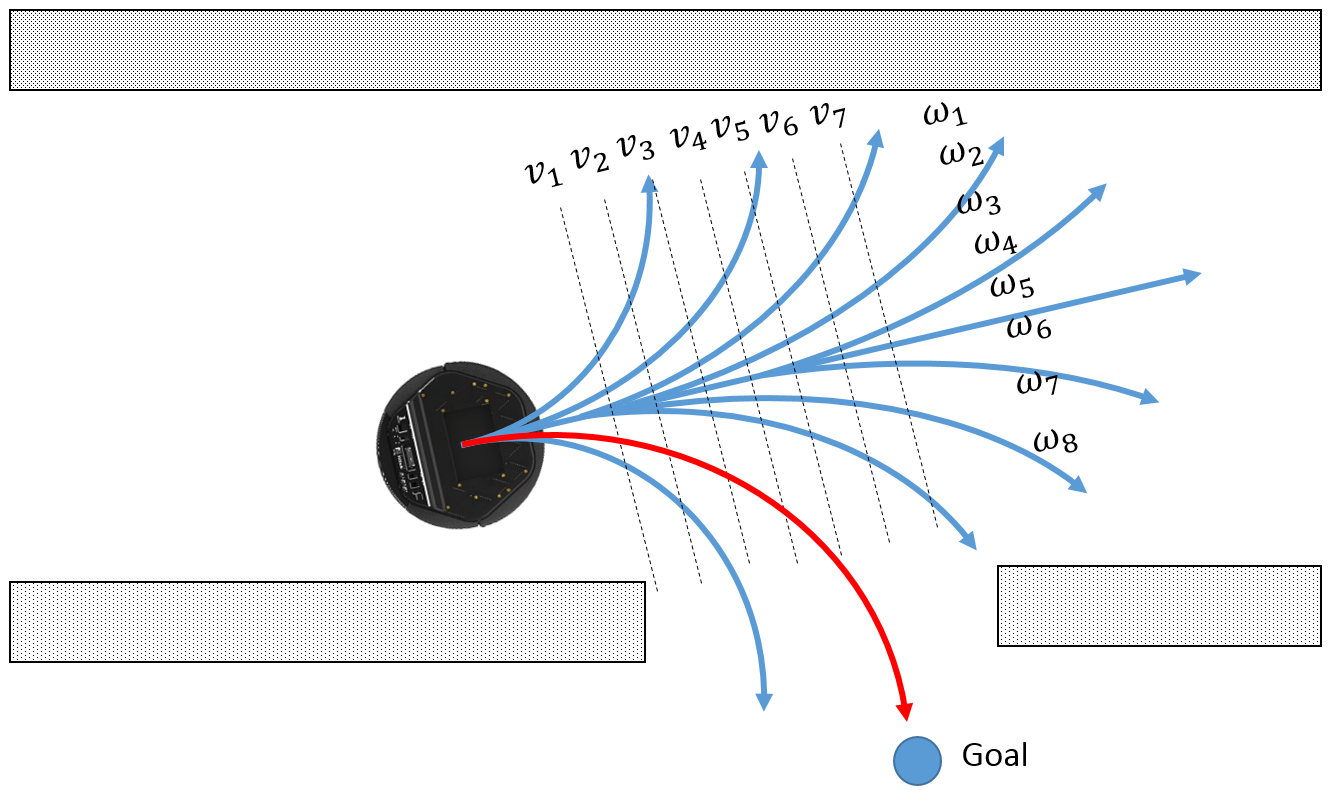
\includegraphics[width=12cm]{pictures/chapter10/pic_10_22.png}
  \caption{並進速度vと回転速度ω}
\end{figure}

% 注1 https://www.openslam.org/gmapping.html
% 注2 http://wiki.ros.org/kobuki
% 注3 https://www.hokuyo-aut.jp/02sensor/07scanner/utm_30lx.html
% 注4 http://wiki.ros.org/tf
% 注5 http://www.openslam.org/gmapping.html
% 注6 The dynamic window approach to collision avoidance、D. Fox、W. Burgard、S. Thrun、Robotics&Automation Magazine、IEEE、vol.4、no.1、pp.23-33、1997
% 注7 http://wiki.ros.org/costmap_2d


%-------------------------------------------------------------------------------
